\documentclass[UTF8]{ctexart}

\usepackage{subfiles}  

%下面的语句, 引入你的头部设置文件
\usepackage{C:/phpStorm_proj/02_myself_ID_EGO/+100_latex_all_math_sel/myPreamble} 
%必须是绝对路径,才能让各个tex在单独编译时使用到


\title{函数}




%------------------------------------------------------------



\begin{document}
	\tableofcontents % 生成目录
	\date{} % 若不写这句, 则默认也会渲染出日期, 所以我们要手动赋空值	
	\maketitle  %这行代码, 让你前面的 title, author, date生效



\part{什么是极限?}

\section{数列的极限}

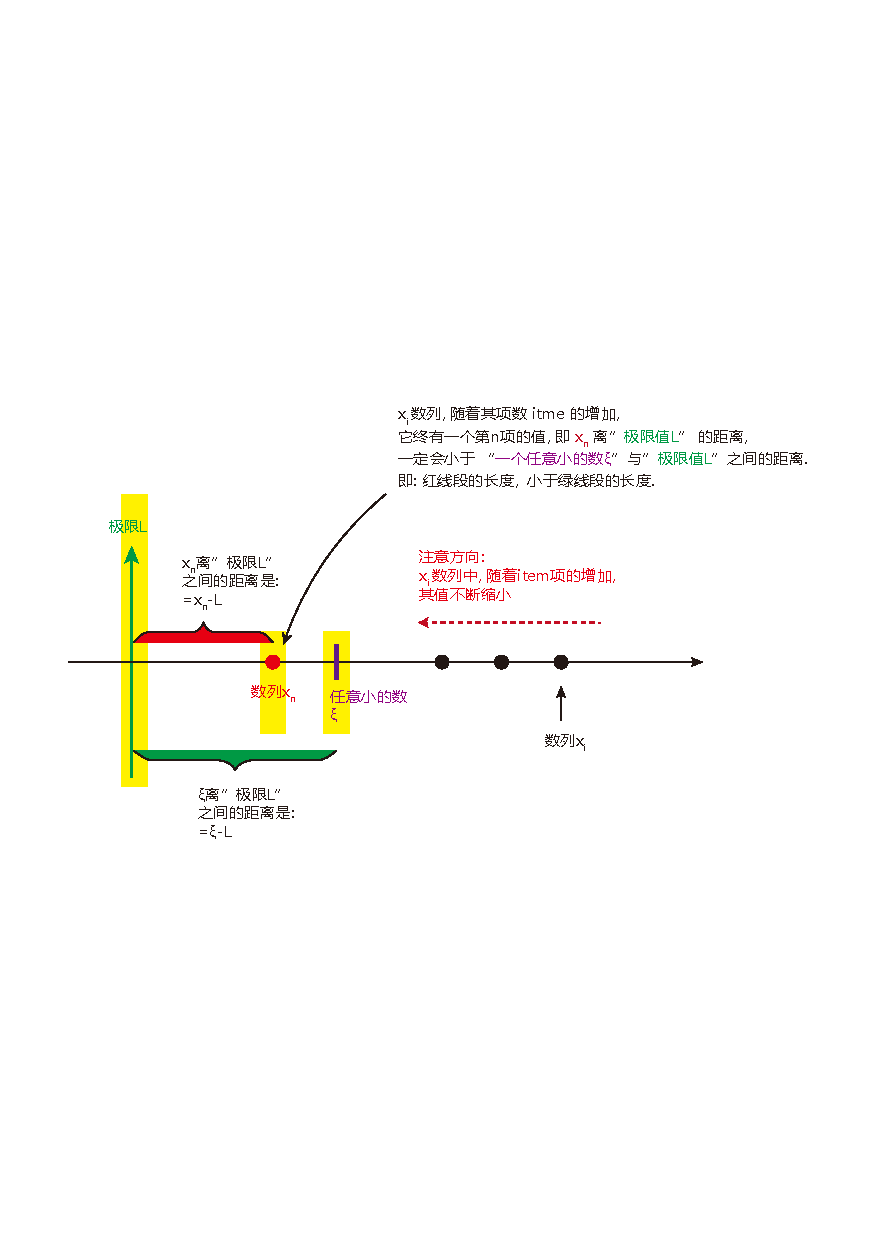
\includegraphics[width=0.9\textwidth]{/0001.pdf}

即: 给定 (1)任意一个极小值$\epsilon $, (2)一个确定的极限值L, (3))一个数列 $ x_i $(里面的元素值不断变小). → 则随着数列 
$ x_i $ 中item的增长, 必定会有一个 item项(比如第n项), 该``item项的值 $ x_n$"与``极限值L"的距离, 必定会小于 ``极小值$\epsilon $"与``极限值L"之间的距离 (这个距离其实就是 $\epsilon $本身). \\



\begin{myEnvSample}
	有数列 $x_n=\dfrac{(-1)^n} {(n+1)^2} $  的极限是0.  问: 该数列取到哪一项item 时, 它与``极限0"之间的距离, 就小于``任意小的数ε"了呢?
	
	即, 问的就是: 该数列与 0 之间的距离, 要小于ε.
	
	
	\[
		\begin{matrix}
			\left| \text{数列}\dfrac{\left( -1 \right) ^n}{\left( n+1 \right) ^2}-\text{极限值}0 \right|<\varepsilon\\
			\left| \dfrac{1}{\left( n+1 \right) ^2} \right|<\varepsilon\\
			\left( n+1 \right) ^2>\dfrac{1}{\varepsilon}\\
			n+1>\dfrac{1}{\sqrt{\varepsilon}}\\
			n>\dfrac{1}{\sqrt{\varepsilon}}-1\\
		\end{matrix}
	\]
	
	为了保证n 为正数(而非有小数点), n就取 $\left( \dfrac{1}{\sqrt{\varepsilon}}-1 \right) +1$	
\end{myEnvSample}




\section{函数的极限}

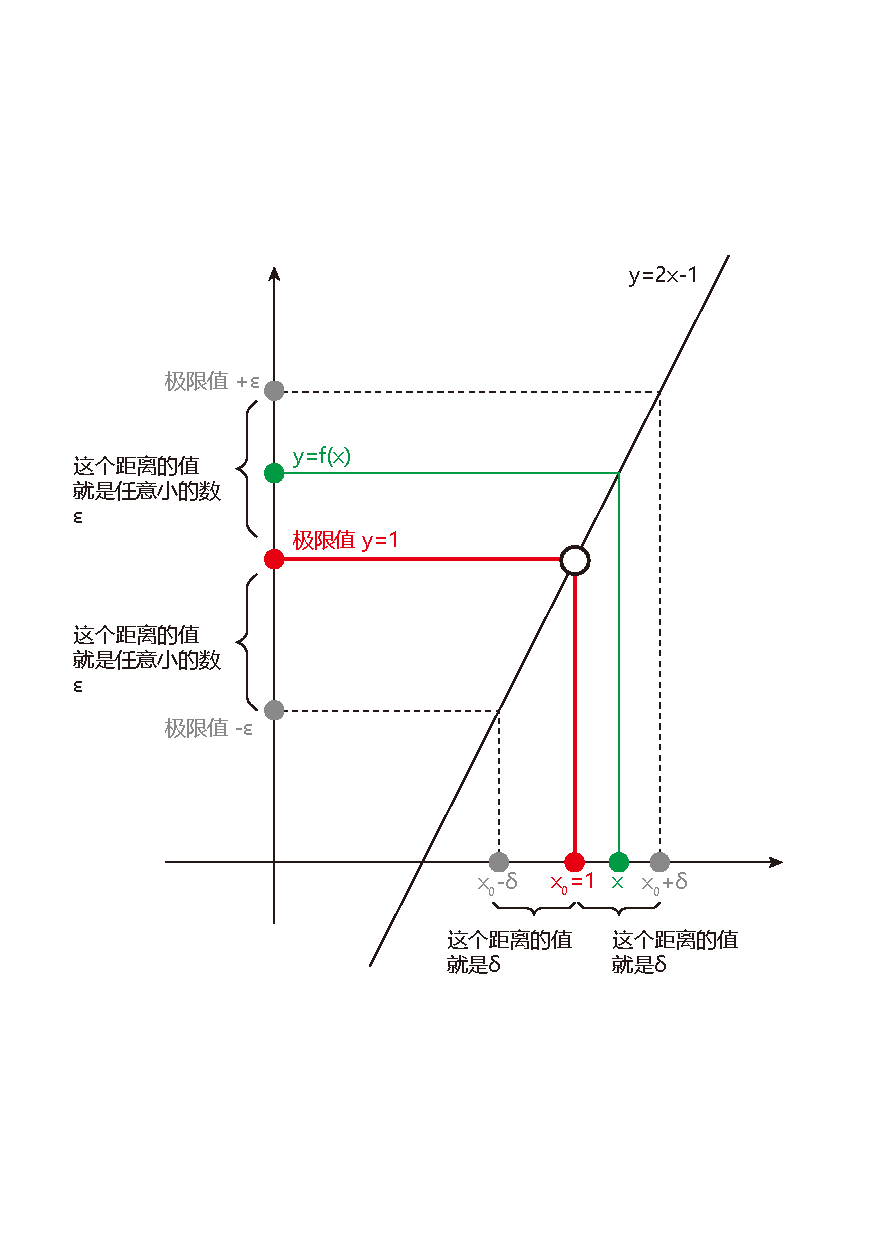
\includegraphics[width=0.6\textwidth]{/0002.pdf}





\part{极限运算法则}

$ \lim (x \pm y) = \lim x \pm \lim y $ \\
$ \lim (x \cdot y) = \lim x \cdot \lim y $  \\
\\
$ \lim (\dfrac{x} {y}) = \dfrac{\lim x} {\lim y} $ \\
$ \lim (\text{常数} C \cdot y) = \text{常数} C \cdot \lim y $ \\
\\
$ \lim y^n = (\lim y)^n $ \\
$ \lim y^{\frac{1} {n}} = (\lim y)^{\frac{1} {n}} $ \\
\\
$ \lim(\text{常数}C) = \text{常数}C $
\\

$\lim_{x\rightarrow a}\left( f\left( x \right) \right) =f\left( a \right) $ \\
$\lim_{x\rightarrow a}\left( \text{常数}C \right) =C$ \\
\\
$ \lim_{x\rightarrow a}\left( f\left( x \right) +g\left( x \right) \right) =\lim_{x\rightarrow a}f\left( x \right) +\lim_{x\rightarrow a}g\left( x \right) $ \\
$\lim_{x\rightarrow a}\left( f\left( x \right) -g\left( x \right) \right) =\lim_{x\rightarrow a}f\left( x \right) -\lim_{x\rightarrow a}g\left( x \right) $ \\
\\
$\lim_{x\rightarrow a}\left( \text{常数}C\cdot f\left( x \right) \right) =\text{常数}C\cdot \lim_{x\rightarrow a}f\left( x \right) $ \\
$\lim_{x\rightarrow a}\left( f\left( x \right) \cdot g\left( x \right) \right) =\lim_{x\rightarrow a}f\left( x \right) \cdot \lim_{x\rightarrow a}g\left( x \right) $ \\
\\
$\lim_{x\rightarrow a}\left( \dfrac{f\left( x \right)}{g\left( x \right)} \right) =\dfrac{\lim_{x\rightarrow a}f\left( x \right)}{\lim_{x\rightarrow a}g\left( x \right)}$ \\
\\
$\lim_{x\rightarrow a}\left( f\left( x \right) \right) ^n=\left( \lim_{x\rightarrow a}f\left( x \right) \right) ^n$ 




~\\
\hrule
~\\


\part{极限的规律, 和求法(方法论)}




\section{若 $ f(x) \textgreater g(x) $, 则 $ \lim f(x) \geq \lim g(x)$  ← 注意: 是大于等于 $\geq$ !}

这个定理也就是说: 虽然 一个函数, 可能大于另一个函数, 但它们的极限, 是有可能相等的. \\

\begin{myEnvSample}
	虽然 $ \dfrac{1} {x} \textgreater \dfrac{1} {x^2}$, 但它们的极限(在 $x \to \infty$ 时), 却是相等的.  即 $ \lim_{n\rightarrow \infty}\dfrac{1}{x}=\lim_{n\rightarrow \infty}\dfrac{1}{x^2}=0
	$ 
	\\
	
	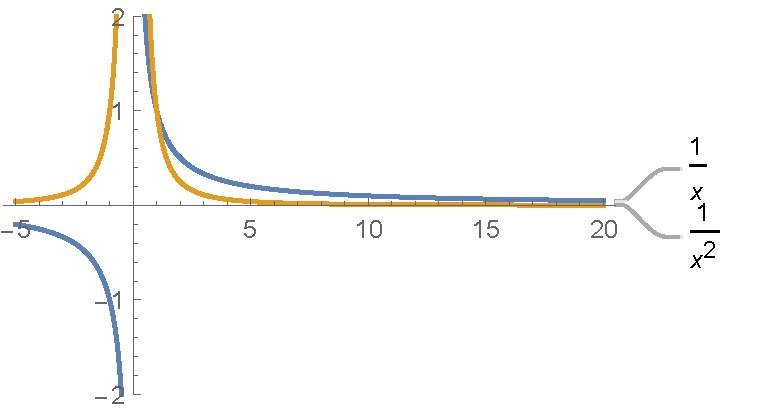
\includegraphics[width=0.5\textwidth]{/0003.pdf}
\end{myEnvSample}




\section{分子上``项的最高次数" \textgreater 分母上``项的最高次数", 则 该分式的极限= ∞. 反之, 则极限=0}

一个函数若是``分数" $ \dfrac{a \cdot x^m}{b \cdot x^n} $, 则其极限, 只看它分子分母上的``最高次数"的情况:






\subsection{对于 $ \dfrac{a \cdot x^m}{b \cdot x^n} $, 若 m \textgreater n, 即: 分子的值 \textgreater 分母的值. 则函数极限值 = ∞}






\subsection{对于 $ \dfrac{a \cdot x^m}{b \cdot x^n} $, 若 m=n, 则函数极限值 = $ \dfrac{a} {b}$}

\begin{myEnvSample}
	\begin{align*}  % 支持每行编号. 若不需要编号, 就用 align*环境
			\lim_{x\rightarrow \infty}\frac{3x^3+4x^2+2}{7x^3+5x^2-3}=\underset{\text{把分子分母,\ 同时除以最高项的}x^3}{\underbrace{\lim_{x\rightarrow \infty}\frac{\frac{3x^3+4x^2+2}{x^3}}{\frac{7x^3+5x^2-3}{x^3}}}}=\underset{\text{把}x\rightarrow \infty \text{代入每一项中}}{\underbrace{\lim_{x\rightarrow \infty}\frac{3+\frac{4}{x}+\frac{2}{x^3}}{7+\frac{5}{x}-\frac{3}{x^3}}}}=\frac{3+0-0}{7-0+0}=\frac{3}{7}\\
		\end{align*}
	
	规律: 当满足 ①  $x \rightarrow \infty$, ② 分子分母的最高次的次数相同, 比如本例最高都是 $x^3$ 次, 则: 极限值, 就取分子分母最高次的系数之比. 如 本例就取 $\dfrac{3 x^3} {7 x^3}$ 的系数, 即 $3/7$ , 这个就是极限值了.
\end{myEnvSample}




\subsection{对于 $ \dfrac{a \cdot x^m}{b \cdot x^n} $, 若 n \textgreater m, 即: 分子的值 \textless 分母的值. 则函数极限值=0}

\begin{myEnvSample}
	\begin{align*}  % 支持每行编号. 若不需要编号, 就用 align*环境
			\lim_{x\rightarrow \infty}\frac{3x^2-2x-1}{2x^3-x^2+5}=\underset{\text{把分子分母,\ 同时除以最高项的}x^3}{\underbrace{\lim_{x\rightarrow \infty}\frac{\frac{3x^2-2x-1}{x^3}}{\frac{2x^3-x^2+5}{x^3}}}}=\underset{\text{把}x\rightarrow \infty \text{代入每一项中}}{\underbrace{\lim_{x\rightarrow \infty}\frac{\frac{3}{x}+\frac{2}{x^2}-\frac{1}{x^3}}{2-\frac{1}{x}+\frac{5}{x^3}}}}=\frac{0+0-0}{2-0+0}=0\\
	\end{align*}

	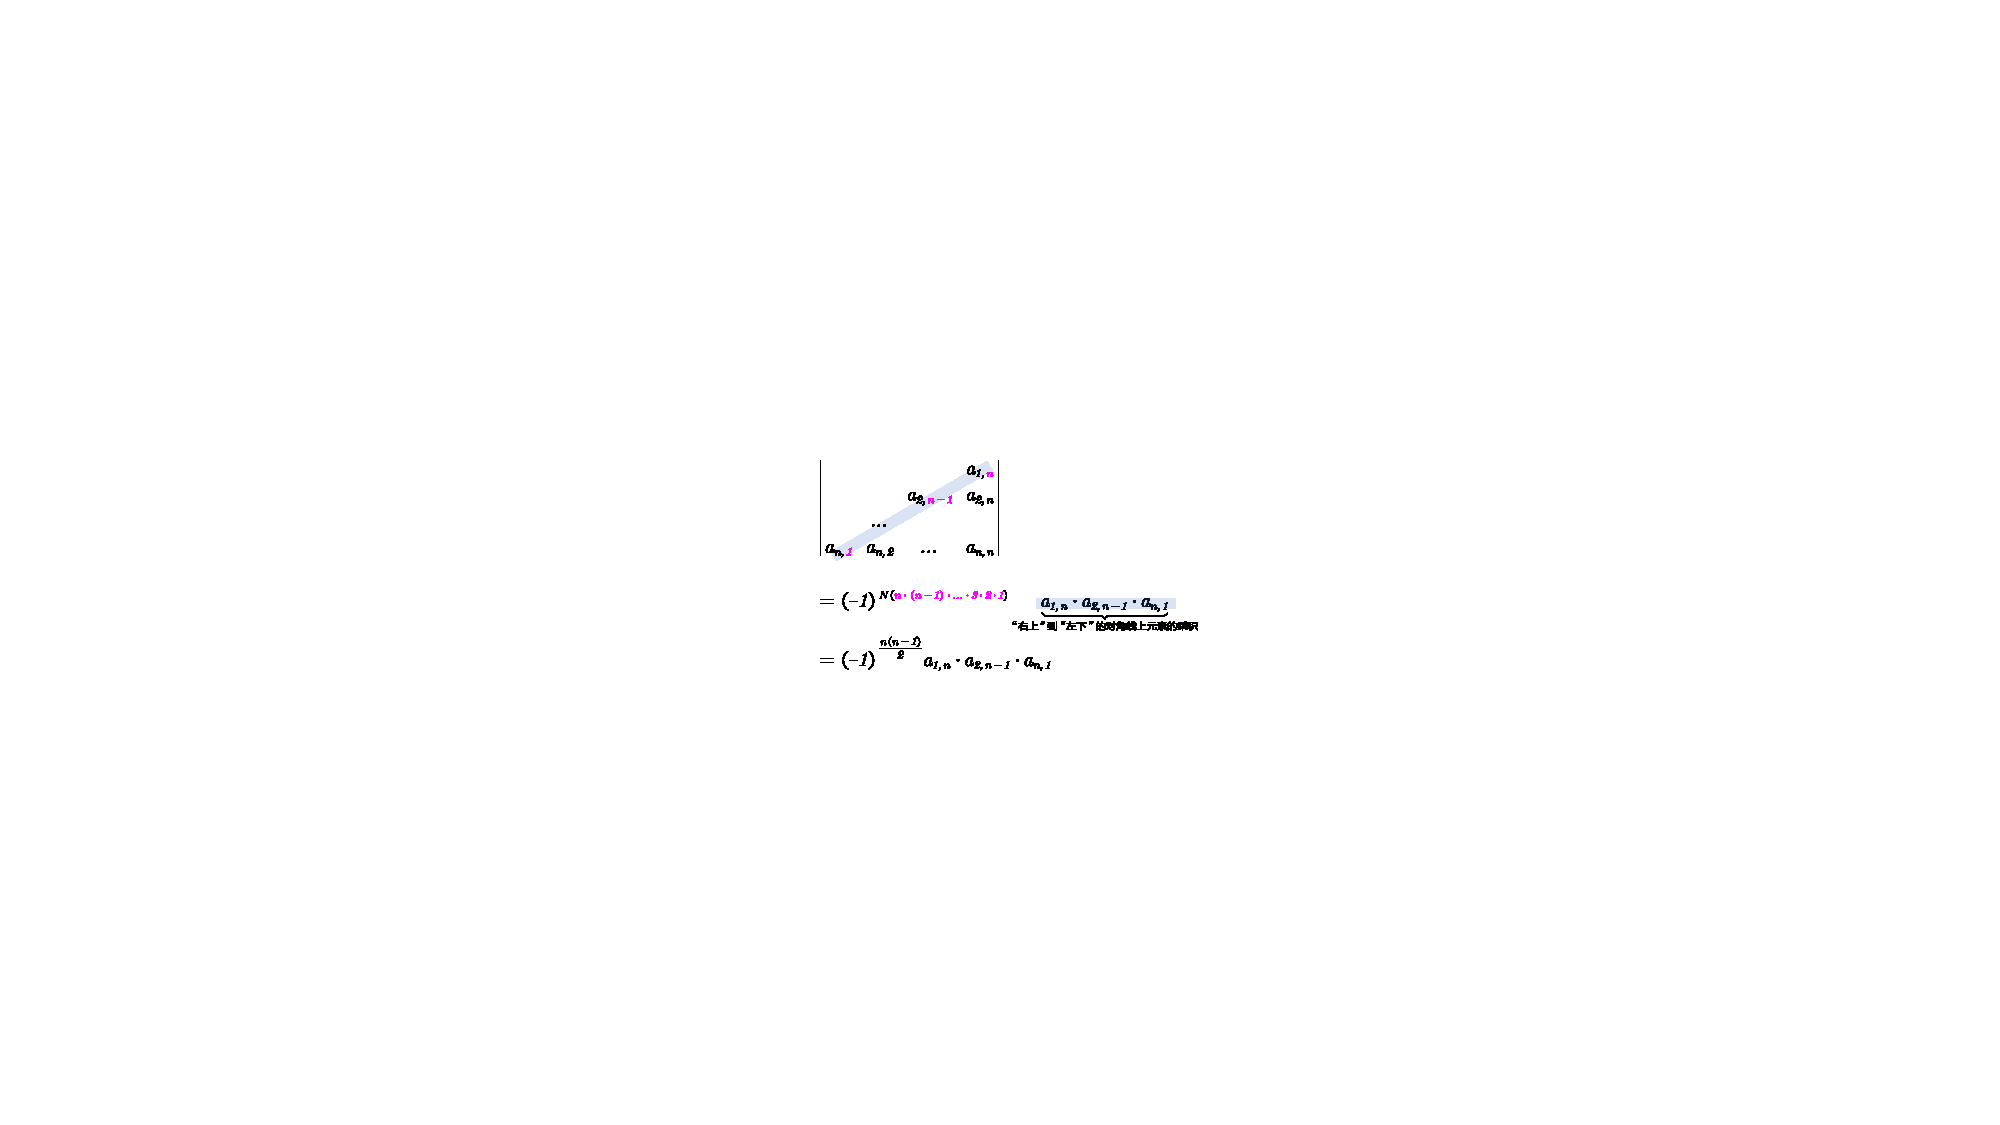
\includegraphics[width=0.5\textwidth]{/0004.pdf}
	
	规律: 当满足 ① $x \rightarrow \infty$, ②分母的最高次的次数, 要比分子的最高次次数还大时, 比如本例``分母的最高次次数"是 $x^3$, 而``分子的最高次次数"只有 $x^2$, 则: 极限就是0.
\end{myEnvSample}



\section{ 重要极限: $\lim_{x \to 0} \dfrac{\sin x} {x} = 1 $}

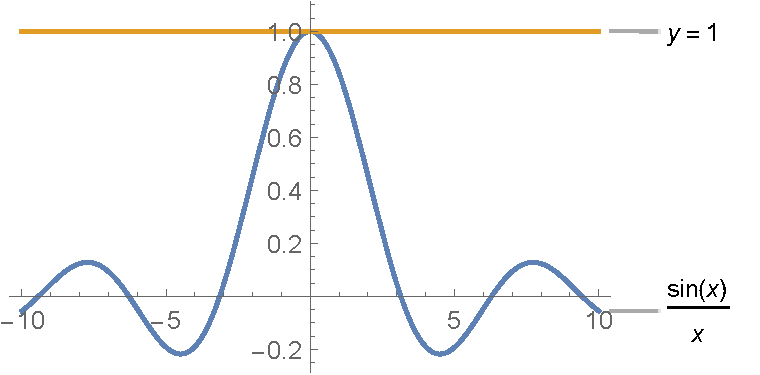
\includegraphics[width=0.5\textwidth]{/0005.pdf}

其实, 它的骨架本质, 是这种形式的: \hl{$\lim_{\Box \to 0} \dfrac{sin \Box} {\Box}$}




\section{重要极限: $ \lim_{x \to \infty} (1+ \dfrac{1} {x})^x = e $}

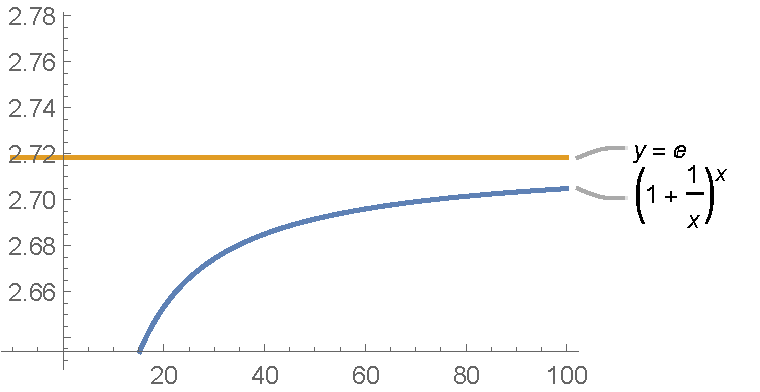
\includegraphics[width=0.5\textwidth]{/0006.pdf}

这个公式其实就是``复利"的终值计算公式: $ \lim_{n \to \infty} (1+ \dfrac{1} {n})^n = e \approx 2.71828 $

注意: 该公式的本质是: \hl{$\lim_{n \to \infty} (1+ \dfrac{1} {\Box})^\Box = e$}.  ← 即两个"方框□"处的数字必须完全相同!

注意: 使用该极限公式时, 中间必须是加号+. 如果题目给出的不是加号, 你也要把它先变换成加号.
	
即: 

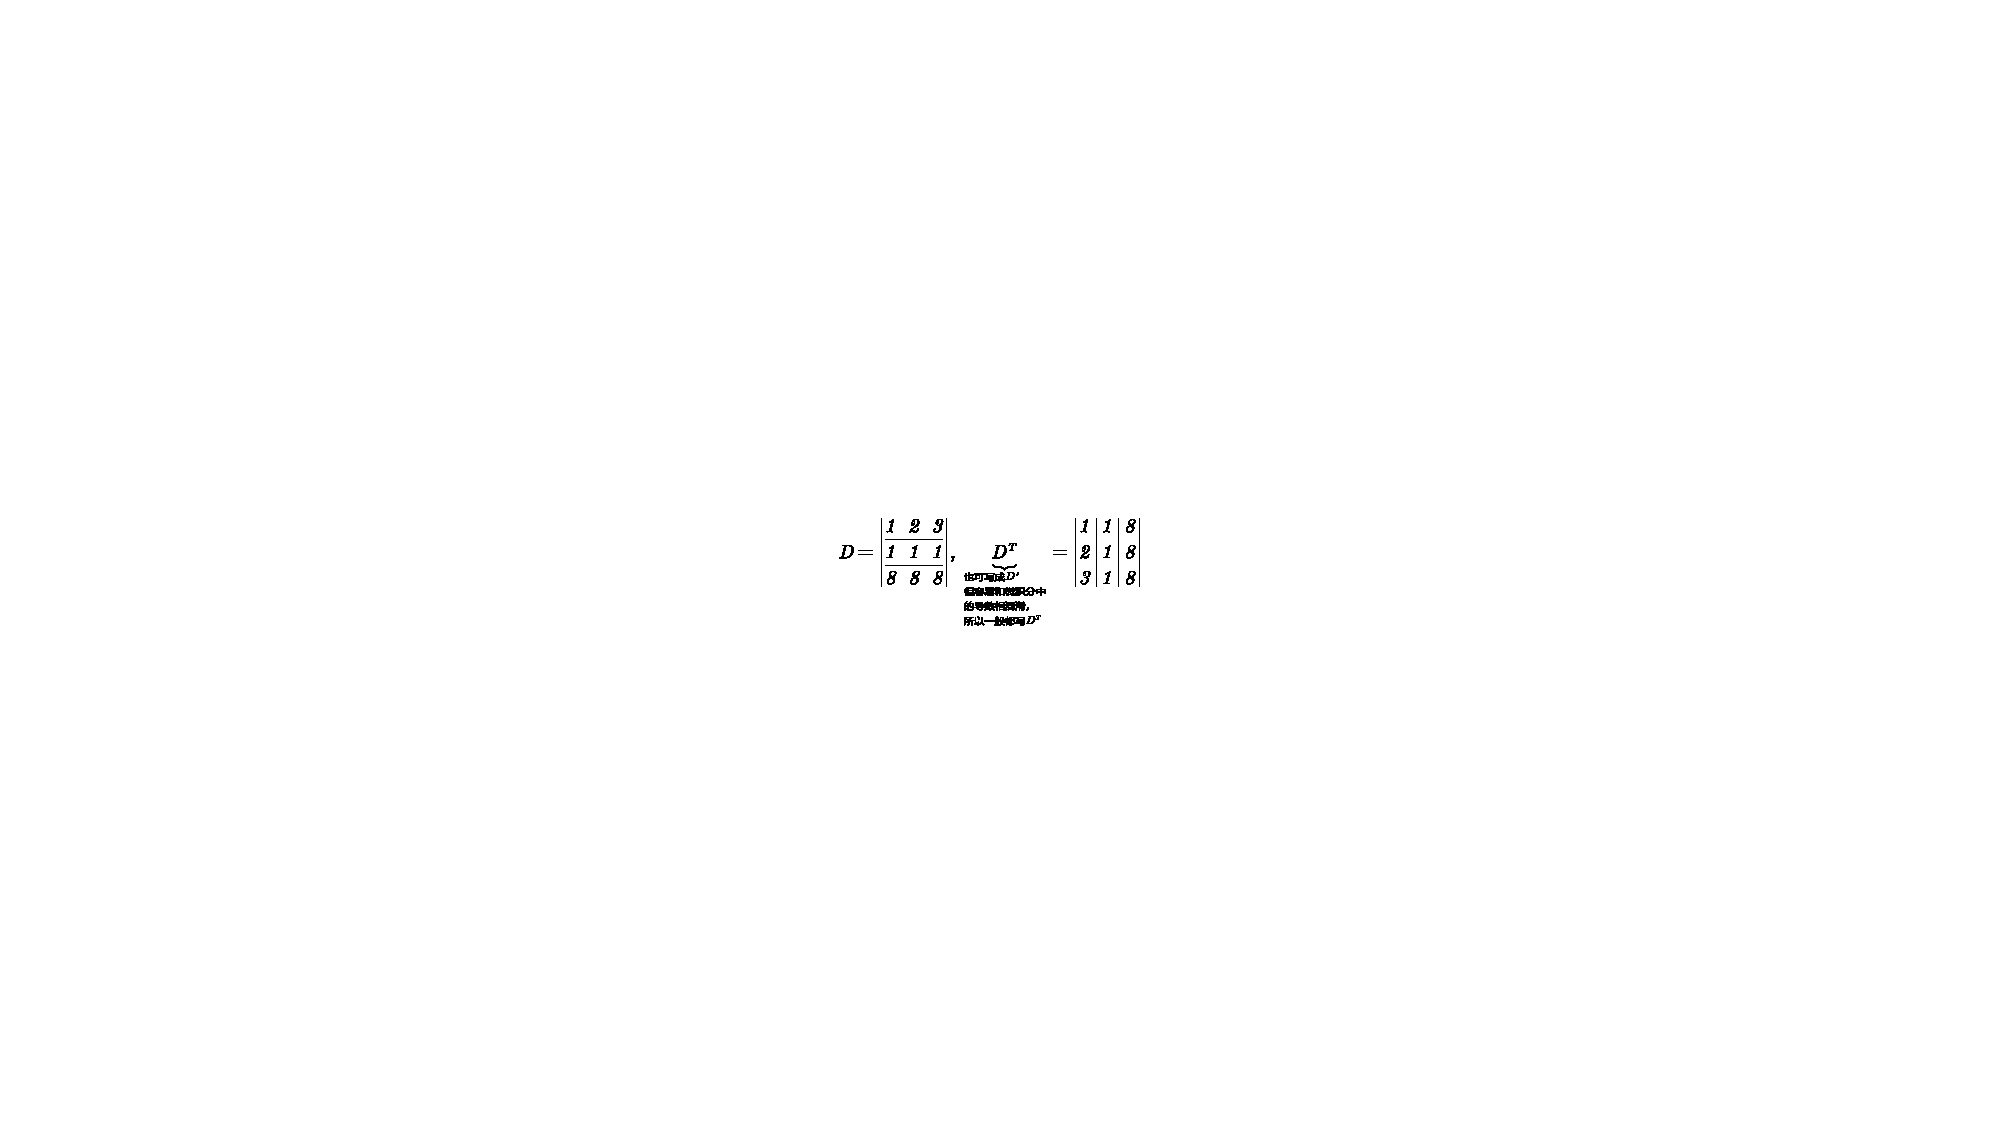
\includegraphics[width=0.3\textwidth]{/0007.pdf}




\begin{myEnvSample}
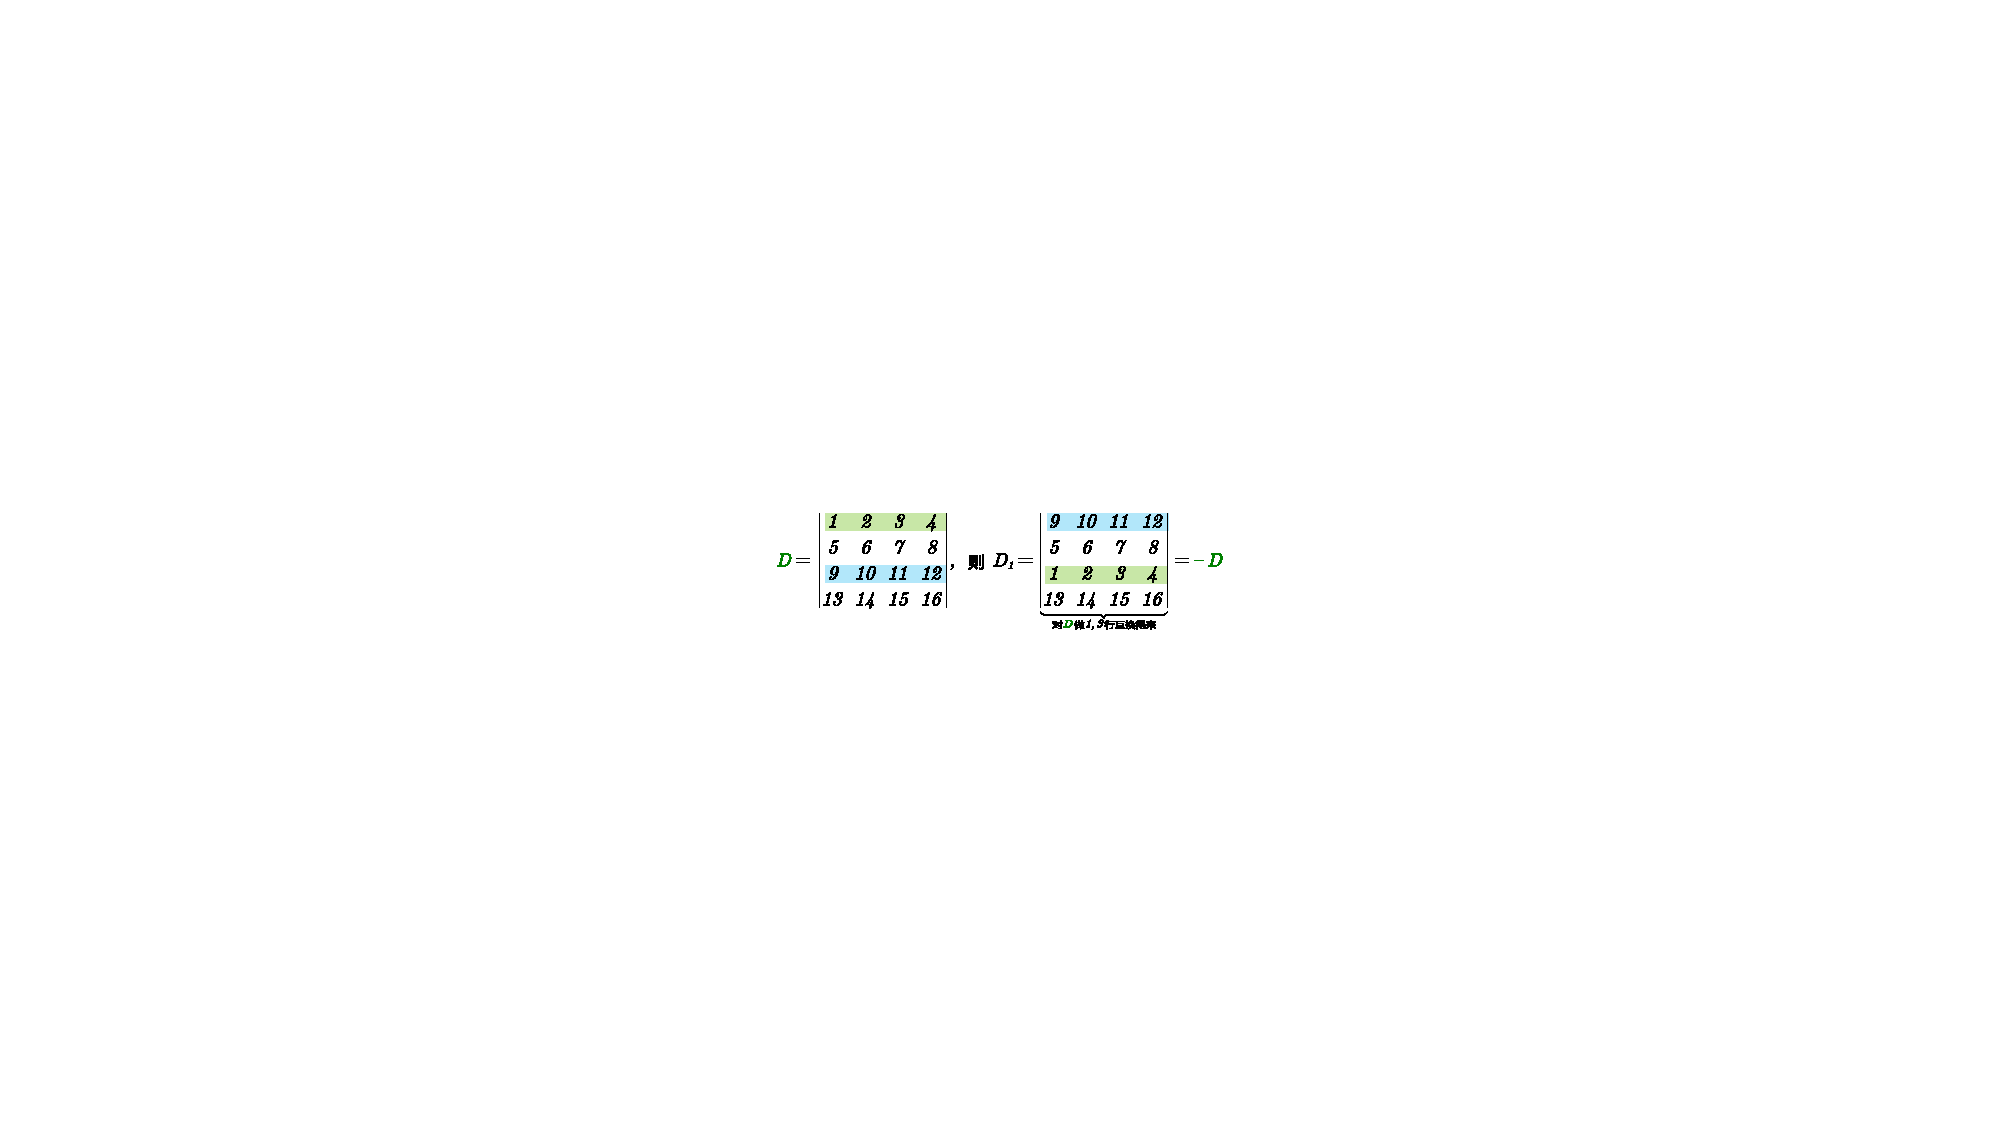
\includegraphics[width=1\textwidth]{/0008.pdf}

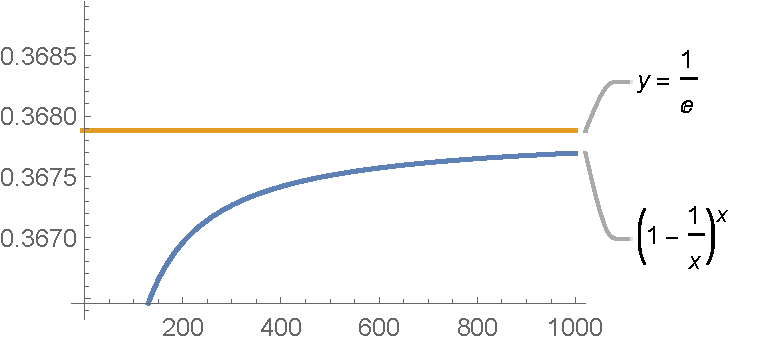
\includegraphics[width=0.5\textwidth]{/0009.pdf}
\end{myEnvSample}



\begin{myEnvSample}
	\begin{align*}  % 支持每行编号. 若不需要编号, 就用 align*环境
		&\lim_{\text{x}\rightarrow \infty}\left( 2+\frac{1}{\text{x}} \right) ^{\text{x}}\ \gets \ \text{这里的2,\ 必须变成1,\ 才能套用公式}\\
	&=\lim_{\text{x}\rightarrow \infty}\left( 2\left( 1+\frac{1}{2\text{x}} \right) \right) ^{\text{x}}=2^{\text{x}}\lim_{\text{x}\rightarrow \infty}\left( 1+\frac{1}{2\text{x}} \right) ^{2\text{x}\cdot \frac{1}{2}}=2^{\text{x}}\underset{\text{这块的极限值,\ 就是e}}{\underbrace{\left[ \lim_{\text{x}\rightarrow \infty}\left( 1+\frac{1}{2\text{x}} \right) ^{2\text{x}} \right] }}^{\frac{1}{2}}=2^{\text{x}}\text{e}^{\frac{1}{2}}
	\end{align*}

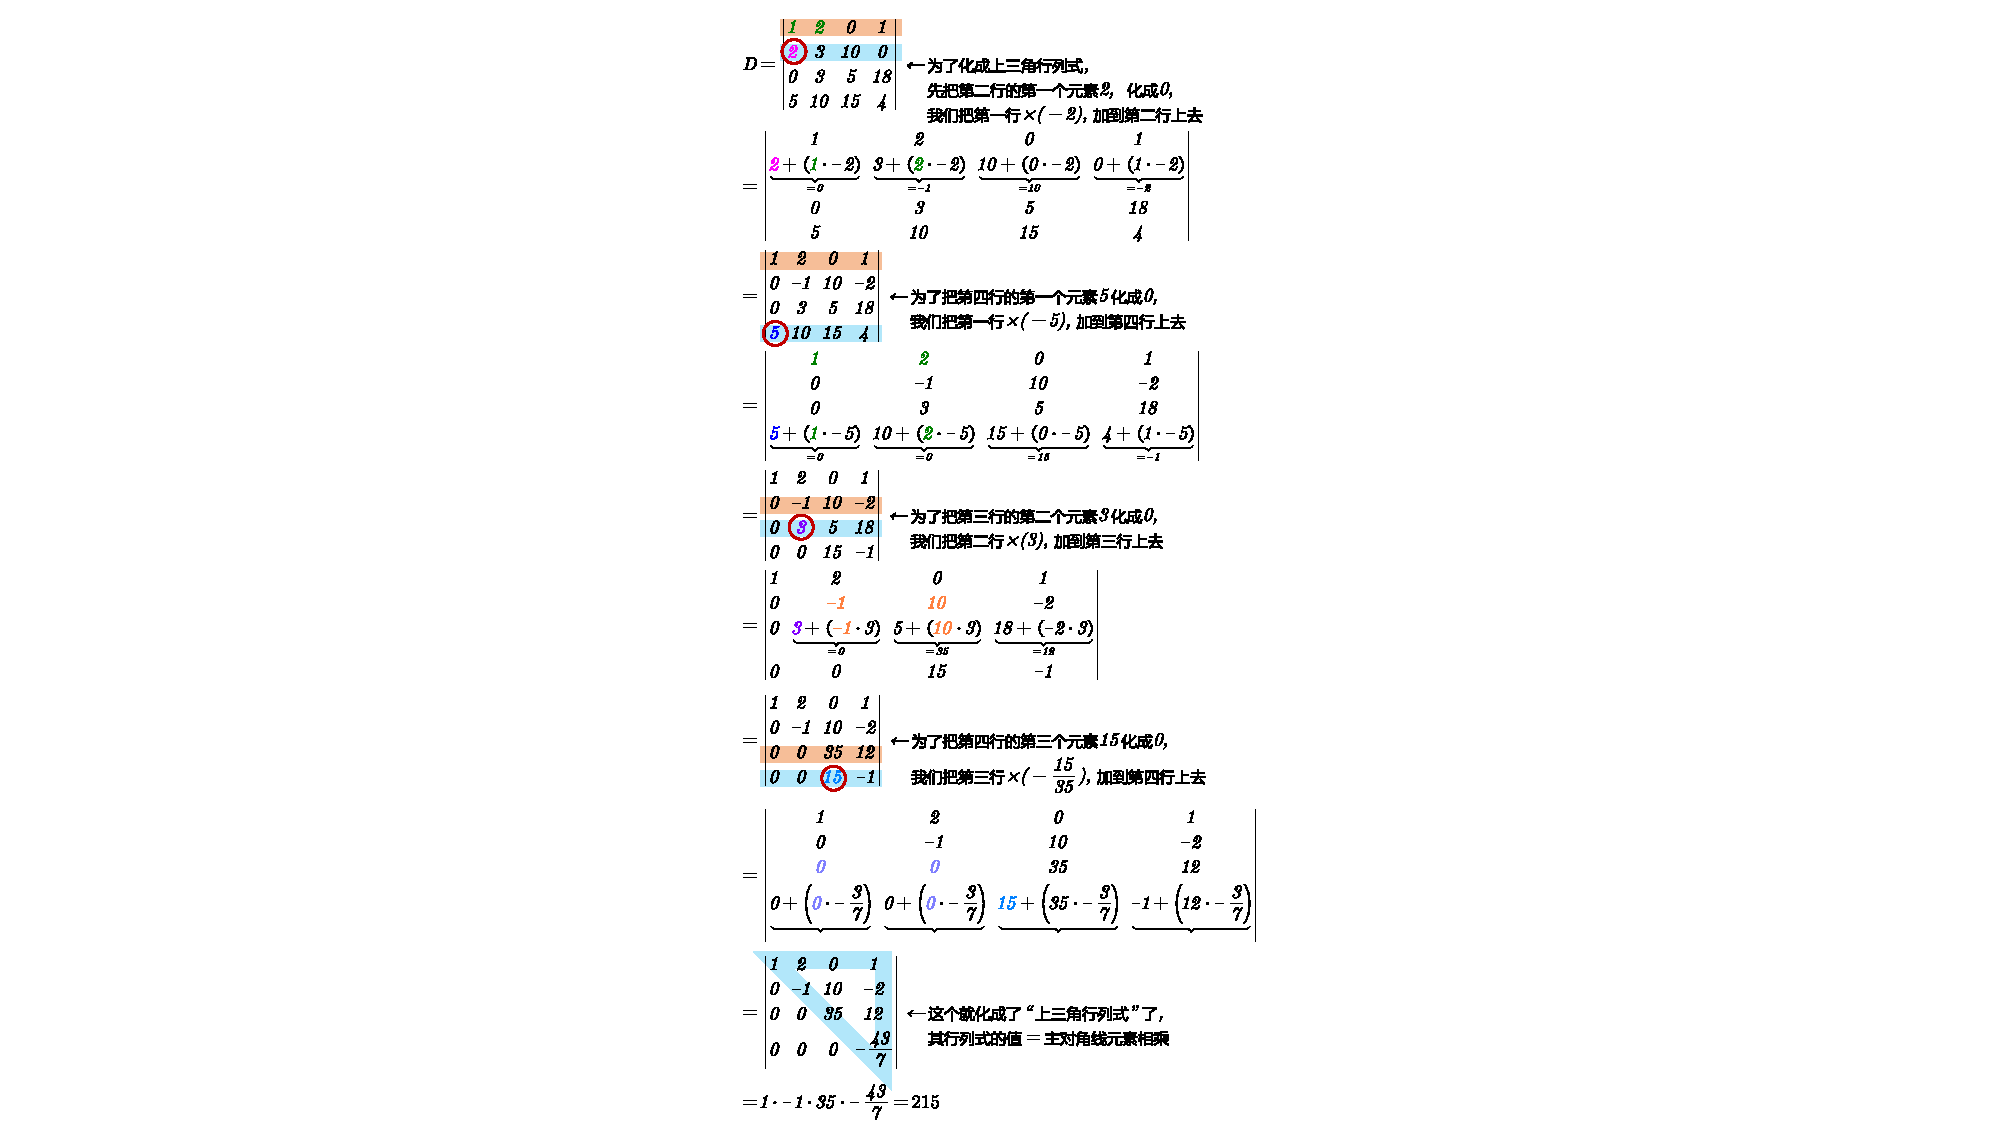
\includegraphics[width=0.5\textwidth]{/0010.pdf}
\end{myEnvSample}



\begin{myEnvSample}
	\begin{align*}  % 支持每行编号. 若不需要编号, 就用 align*环境
		&\lim_{\text{x}\rightarrow \infty}\left( 1+\frac{5}{\text{x}} \right) ^{\text{x}}\ \gets \ \text{这里分子上的5,\ 必须变成1,\ 才能套用公式}\\
		&=\lim_{\text{x}\rightarrow \infty}\left( 1+\frac{1}{\frac{\text{x}}{5}} \right) ^{\text{x}}=\lim_{\text{x}\rightarrow \infty}\left( 1+\frac{1}{\frac{\text{x}}{5}} \right) ^{\frac{\text{x}}{5}\cdot 5}=\underset{\text{这块的极限值,\ 就是e}}{\underbrace{\left[ \lim_{\text{x}\rightarrow \infty}\left( 1+\frac{1}{\frac{\text{x}}{5}} \right) ^{\frac{\text{x}}{5}} \right] }}^5=\text{e}^5\\
	\end{align*}
	
	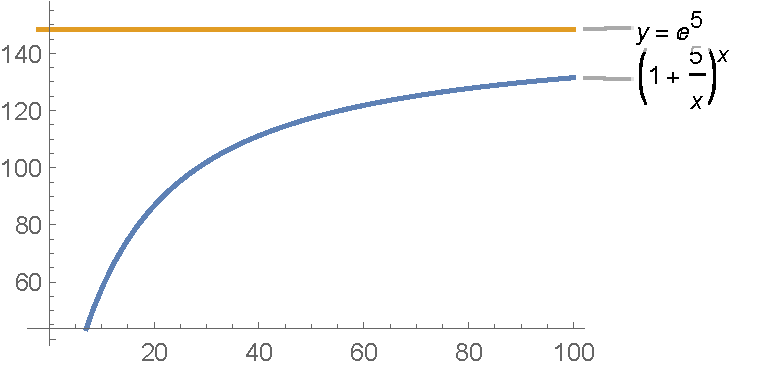
\includegraphics[width=0.5\textwidth]{/0011.pdf}
\end{myEnvSample}





\section{重要极限: $ \lim_{x \to 0} (1+x)^{\frac{1} {x}} =e $}

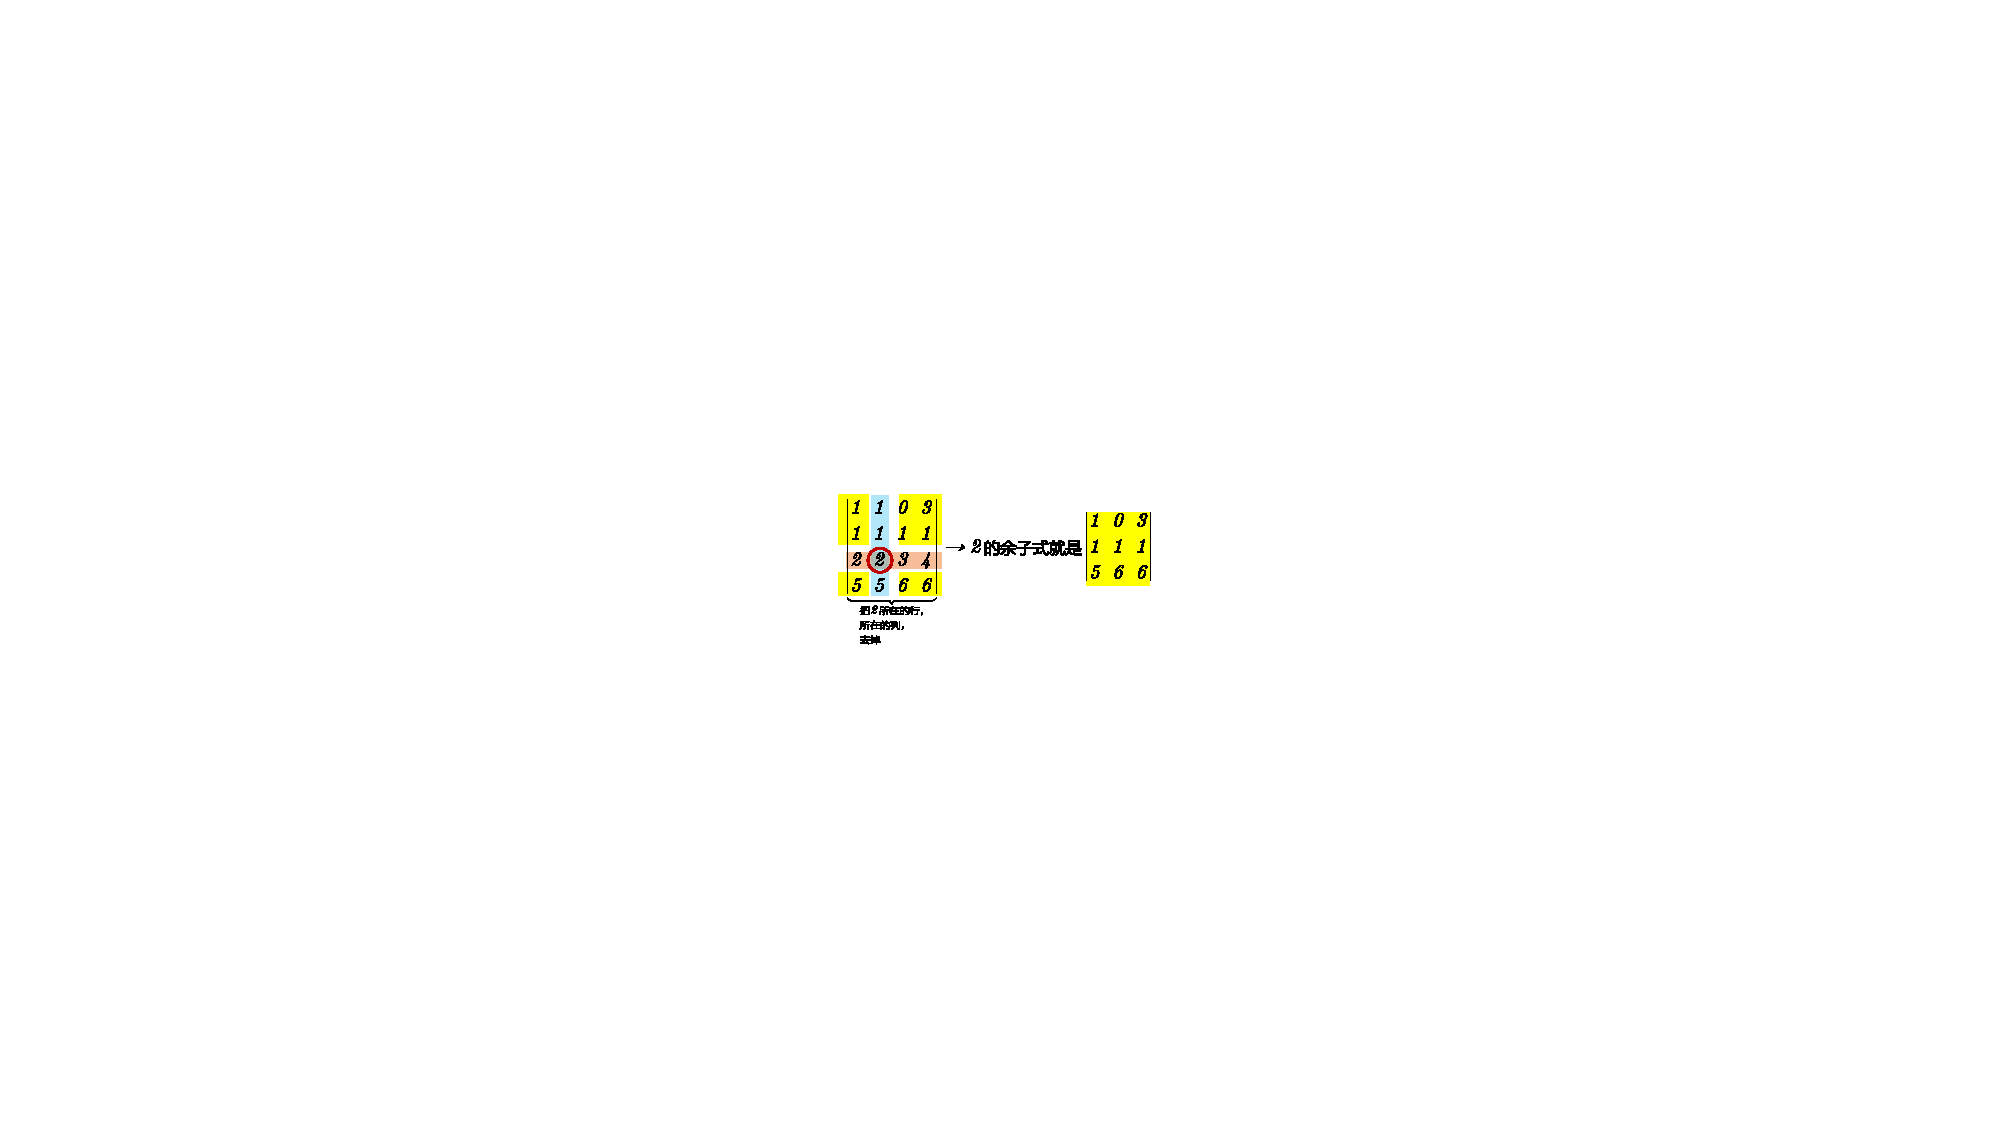
\includegraphics[width=0.5\textwidth]{/0012.pdf}





\section{求极限时, 遇到 $ \dfrac{0}{0}$ 或 $\dfrac{\infty} {\infty}$ 这种时, 可使用``洛必达法则" : 
	$	\lim_{x → a}\dfrac{f(x)}{F(x)}=\lim_{x\rightarrow a}\dfrac{f'(x)}{F'(x)}$}

洛必达法则  L'Hospital's rule , 主要用于求极限, 尤其是 $ \dfrac{0}{0}, \dfrac{\infty} {\infty}$ 这种的.

两个无穷小之比$ \dfrac{0}{0}$, 或两个无穷大之比 $\dfrac{\infty} {\infty}$ 的极限可能存在,也可能不存在。因此,求这类极限时, 往往需要适当的变形,转化成可利用``极限运算法则"或``重要极限的形式", 进行计算. 洛必达法则, 便是应用于这类极限计算的通用方法. \\

洛必达法则的内容: 

有两个函数 f(x) 和 F(x), 若它们满足这些条件:

(1) 当 $x \to a$ 时, 有 f(x) 和 F(x)的值, 都趋向于0.

(2) 在a的``去心邻域"内,  f'(x) 和 F'(x) , 即它们的导数均存在, 且 F'(x) $\ne 0$

(3) 当$x \to a$ 时, 有 $\lim_{x \to a} \dfrac{f'(x)} {F'(x)}$ 的值存在, 或其极限值 = 无穷大 ($\pm \infty$皆可) \\

则, 而我们就有这个结论:

当$x \to a$ 时, 这两个函数的比值, 即 \hl{$\lim_{x \to a} \dfrac{f(x)} {F(x)} = \lim_{x \to a} \dfrac{f'(x)} {F'(x)}$} =存在, 或=$\pm \infty$ \\

总结就是:

- 如果``这两个函数的导数之比"的极限值存在, 则它们的"函数之比"的极限, 也存在, 且其值就等于前者.  即: 若 $\lim_{x \to a} \dfrac{f'(x)} {F'(x)} $ 存在, 则  $\lim_{x \to a} \dfrac{f(x)} {F(x)} = \lim_{x \to a} \dfrac{f'(x)} {F'(x)}$

- 如果 $\lim_{x \to a} \dfrac{f'(x)} {F'(x)} $ 这个极限值 = $\infty$, 则   $\lim_{x \to a} \dfrac{f(x)} {F(x)} $ 也= $\infty$

- \underline{如果 $\lim_{x \to a} \dfrac{f'(x)} {F'(x)} $ 这个极限值不存在, 则本``洛必达法则"方法无效}, 就要使用其他方法来求该极限了.


\begin{myEnvSample}
	求 \begin{align*}  % 支持每行编号. 若不需要编号, 就用 align*环境
		\lim_{x\rightarrow 0}\frac{\sin\text{\ }ax}{\sin\text{\ }bx}\ \left( b\ne 0 \right) 
	\end{align*}
	
	先看``它们的导数之比"的极限, 存不存在?
	
	$$
	\lim_{x\rightarrow 0}\frac{\left( \sin ax \right) '}{\left( \sin bx \right) '}=\lim_{x\rightarrow 0}\frac{\left( \cos ax \right) \cdot a}{\left( \cos bx \right) \cdot b}=\frac{a}{b}
	$$
	
	其``导数之比"的极限存在, 所以``原函数"之比的极限也存在, 即当 $x \to 0$时, 就= $\dfrac{a}{b}$ \\
	
	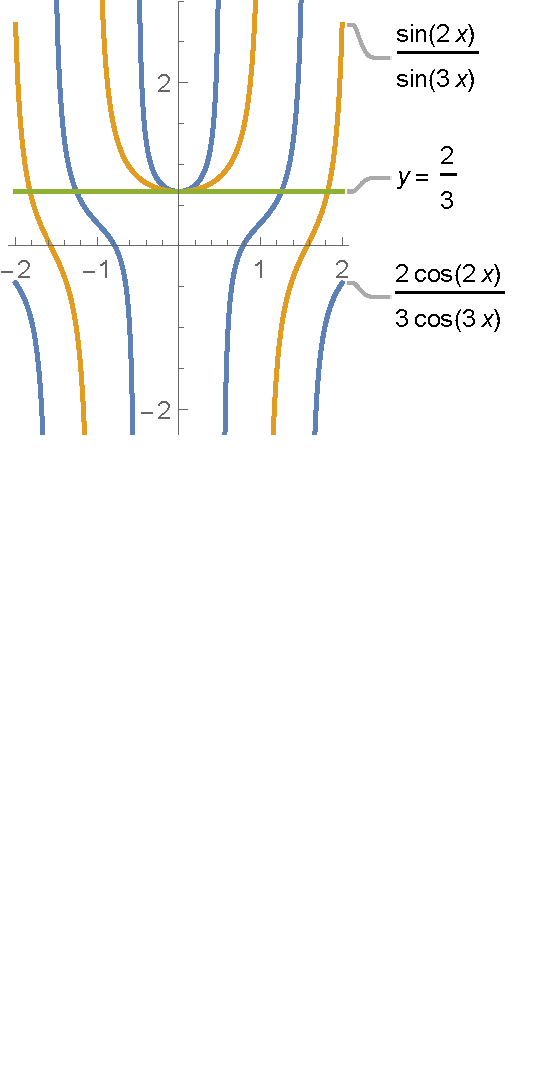
\includegraphics[width=0.4\textwidth]{/0020.pdf}
\end{myEnvSample}



\begin{myEnvSample}
	求 $\lim_{n\rightarrow 1}\dfrac{x^3-3x+2}{x^3-x^2-x+1}$  ← 先把x=1代入进去,发现满足$\dfrac{0}{0}$型,能用``洛必达法则". 那么我们就先来求``这两个函数的导数之比"的极限:
	
	$ =\lim_{n\rightarrow 1}\dfrac{\left( x^3-3x+2 \right) '}{\left( x^3-x^2-x+1 \right) '}=\lim_{n\rightarrow 1}\dfrac{3x^2-3}{3x^2-2x-1} $ ← 再把 x=1代入进去,发现满足$\dfrac{0}{0}$型, 继续能用``洛必达法则"
	
	$=\lim_{n\rightarrow 1}\dfrac{\left( 3x^2-3 \right) '}{\left( 3x^2-2x-1 \right) '}=\lim_{n\rightarrow 1}\dfrac{6x}{6x-2} $ ← 再把 x=1代入进去,发现=$\dfrac{6}{4}$, 不满足$\dfrac{0}{0}$型, 或$\dfrac{\infty}{\infty}$型了, 就不能继续用``洛必达法则"了.
	
	所以,本题的最终结果,即 $\lim_{n\rightarrow 1}\dfrac{x^3-3x+2}{x^3-x^2-x+1}=\dfrac{6}{4}=\dfrac{3}{2}$
\end{myEnvSample}  



即: 

(1) 如果你代入x的值后, 发现 ``分子比分母"的极限, 是 $ \dfrac{0} {0}$ 或$ \dfrac{\infty} {\infty}$ 这种不定式极限 (这两种称为``基本型"), 就适合于用``洛必达法则"来求解. 并且, 其他变种, 如: $ 0 \cdot \infty$型, $\infty-\infty$型, $1^{\infty}$型, $\infty^0$型, $0^0$型的极限,  可以通过相应的变换, 转换成上述两种基本的不定式形式, 来求解.

(2) 不过在使用``洛必达法则"之前, 还需要验证一下: 分子分母在限定的区域内, 是否分别``可导". 满足的话, 才能用``洛必达法则".

(3) 使用了一次``洛必达法则"后, 如果极限依然不确定是否存在,即结果仍然为``未定式",就再在验证前面所说的两个条件的基础上, 继续使用"洛必达法则"来做.  即, 若条件符合,``洛必达法则"可连续多次使用,直到求出极限为止. \\


\begin{myEnvSample}
	\begin{align*}  % 支持每行编号. 若不需要编号, 就用 align*环境
		&\lim_{x\rightarrow 0}\frac{}{x^3}\ \gets \frac{0}{0}\text{型,用}“\text{洛必达法则}”\\
		&=\lim_{x\rightarrow 0}\frac{\left( x-\sin x \right) '}{\left( x^3 \right) '}=\lim_{x\rightarrow 0}\frac{1-\cos x}{3x^2}\ \gets \frac{0}{0}\text{型,继续用}“\text{洛必达法则}”\\
		&=\lim_{x\rightarrow 0}\frac{\left( 1-\cos x \right) '}{\left( 3x^2 \right) '}=\lim_{x\rightarrow 0}\frac{\sin x}{6x}=\frac{1}{6}\underset{=1}{\underbrace{\lim_{x\rightarrow 0}\frac{\sin x}{x}}}\ \gets \text{根据极限公式,有}\lim_{x\rightarrow 0}\frac{\sin x}{x}=1\\
		&=\frac{1}{6}
	\end{align*}
\end{myEnvSample}




\begin{myEnvSample}
	\begin{align*}  % 支持每行编号. 若不需要编号, 就用 align*环境
		&\begin{matrix}
			\lim_{x\rightarrow \frac{\pi}{2}}\left( \sec x-\tan x \right) \ \gets \infty -\infty \text{型,可用}“\text{洛必达法则}”\\
		\end{matrix}\\
		&=\lim_{x\rightarrow \frac{\pi}{2}}\left( \frac{1}{\cos x}-\frac{\sin x}{\cos x} \right) \ \gets \text{原式先变化成分式的形式}\\
		&=\lim_{x\rightarrow \frac{\pi}{2}}\frac{1-\sin x}{\cos x}=\lim_{x\rightarrow \frac{\pi}{2}}\frac{\left( 1-\sin x \right) '}{\left( \cos x \right) '}\ \gets \text{使用}“\text{洛必达法则}”\\
		&=\lim_{x\rightarrow \frac{\pi}{2}}\frac{-\cos x}{-\sin x}\ \gets \text{在}x\rightarrow \frac{\pi}{2}\text{时,分子}\cos \rightarrow 0,\text{所以整个分数值}\rightarrow 0\\
		&=0
	\end{align*}
	
	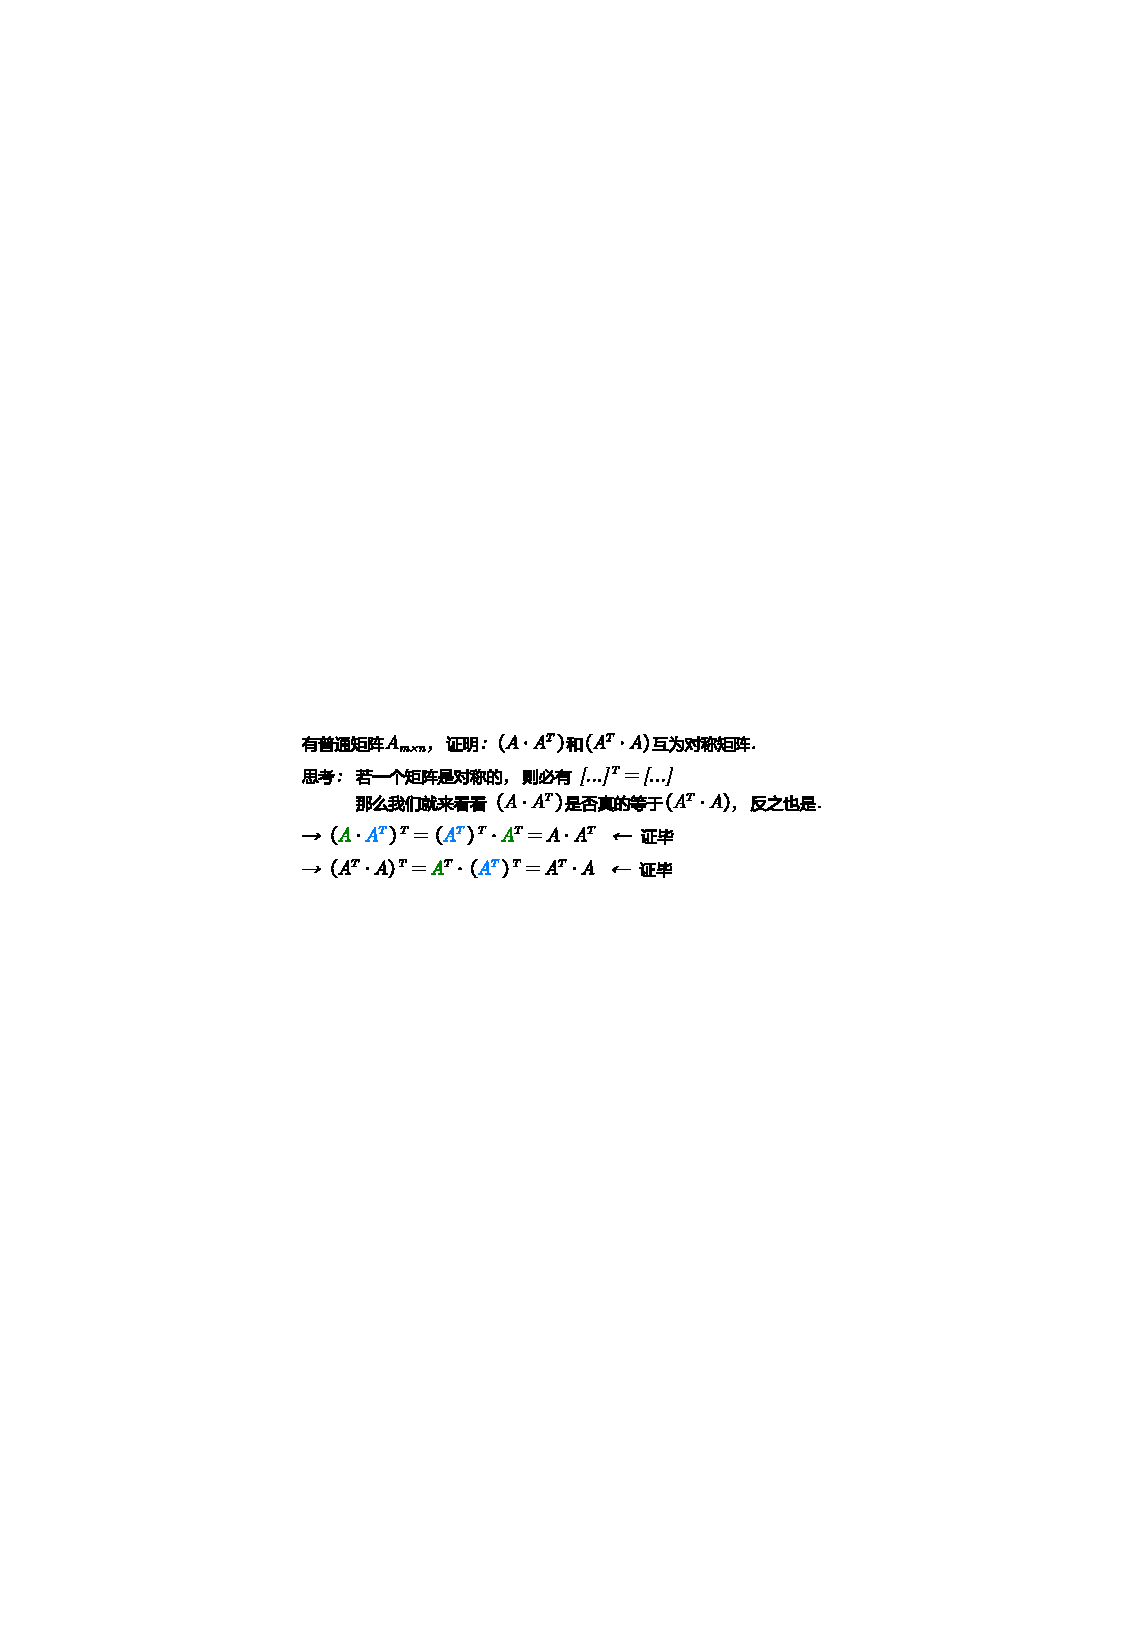
\includegraphics[width=0.5\textwidth]{/0021.pdf}
\end{myEnvSample}




\begin{myEnvSample}
	求 $\lim_{x\rightarrow 0^+}x^x$
	
	如果把 x=0 代入的话, 会得到 $0^0=0^{1-1}=\frac{0^1}{0^1}$, 因为分母不能为0,所以该分式无意义.
	
	虽然 $0^0$ 无意义,但我们可以求它附近的极限处的值.
	
	根据公式: $\boxed{e^{b\ln a}=e^{b\log _ea}=e^{\overset{\text{即\ }e^?=a^b}{\overbrace{\log _ea^b}}}=a^b}$, 即 \hl{$e^{b\ln a}=a^b$}
	
	我们就有: 
	\begin{align*}  % 支持每行编号. 若不需要编号, 就用 align*环境
		&\lim_{x\rightarrow 0^+}{\color{blue}x}^{\color{red}x}=\lim_{x\rightarrow 0^+}e^{{\color{red}x}\ln {\color{blue}x}}\\
		&=\lim_{x\rightarrow 0^+}e^{\frac{\ln x}{x^{-1}}}\ \gets \text{指数上的分式,\ 可以用}“\text{洛必达法则}”\text{做,对分子分母同时求导}\\
		&=\lim_{x\rightarrow 0^+}e^{\frac{x^{-1}}{-1x^{-2}}}=\lim_{x\rightarrow 0^+}e^{-\frac{1}{x^{-1}}}=\lim_{x\rightarrow 0^+}e^{-x}=e^0=1
	\end{align*}
	
	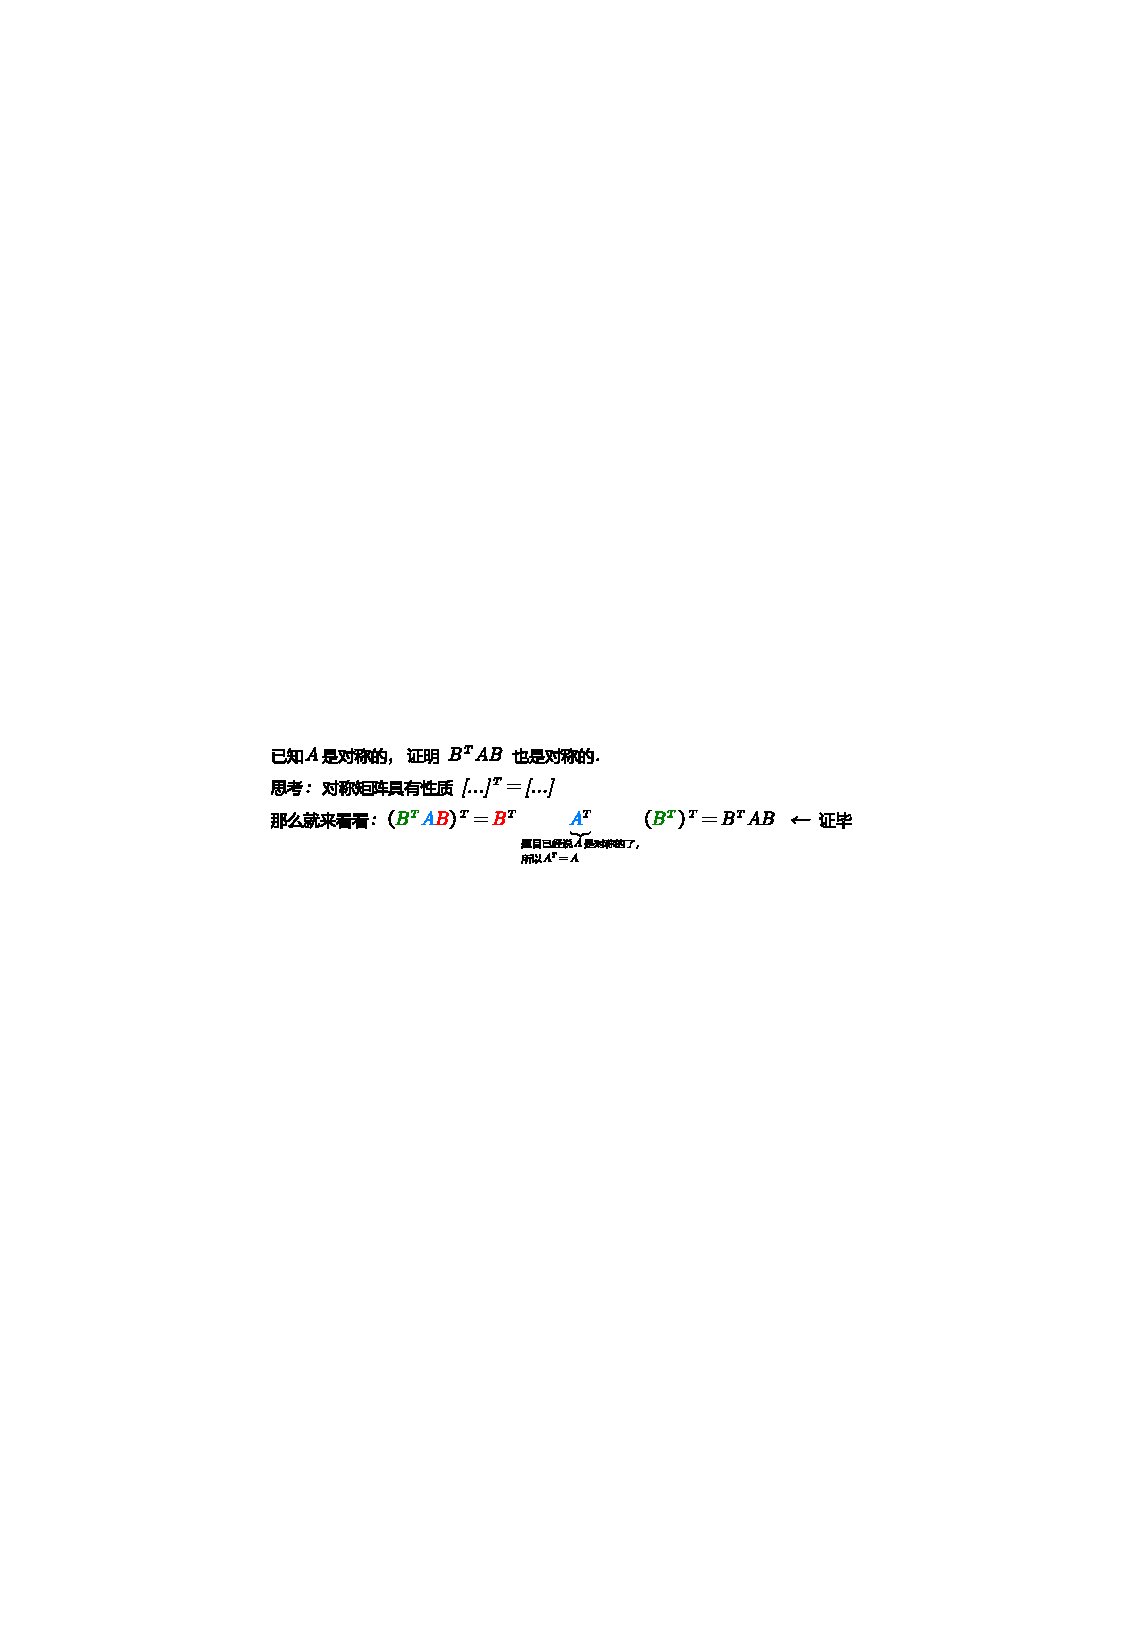
\includegraphics[width=0.5\textwidth]{/0022.pdf}
\end{myEnvSample}





\subsection{技巧1: 在乘积中, 可以用 ``等价无穷小替换"}

下面的例子中, 会用到等价无穷小的替换, 但注意: 只有在``乘积"中, 才能用``等价无穷小替换", 如果是在加减中, 则不能用替换!

\begin{myEnvSample}
\begin{align*}  % 支持每行编号. 若不需要编号, 就用 align*环境
&	\begin{matrix}
	\lim_{x\rightarrow 0}\\
\end{matrix}\frac{\tan x-x}{x^2\underset{\text{可用}x\text{代替}}{\underbrace{\sin x}}}\ \gets \frac{0}{0}\text{型,用}“\text{洛必达法则}”\\
&\text{首先,因为当}x\rightarrow 0\text{时,}\sin x\text{在此处的}y\text{值,等价于}x\text{在此处的}y\text{值,所以我们可以用}x\text{来代替}\sin x\\
&=\begin{matrix}
	\lim_{x\rightarrow 0}\\
\end{matrix}\frac{\tan x-x}{x^2x}=\begin{matrix}
	\lim_{x\rightarrow 0}\\
\end{matrix}\frac{\left( \tan x-x \right) '}{\left( x^3 \right) '}\ \gets \text{用}“\text{洛必达法则}”\\
&=\begin{matrix}
	\lim_{x\rightarrow 0}\\
\end{matrix}\frac{\sec ^2x-1}{3x^2}\ \gets \frac{0}{0}\text{型,继续用}“\text{洛必达法则}”\\
&=...\\
\end{align*}
\end{myEnvSample}




\subsection{技巧2: 趋近于``常数"的那些项, 就向外挪出去, 而不要一并进入求导环节}


\begin{myEnvSample}
比如, $ \lim_{x\rightarrow 0} \dfrac{x^2-\tan x}{\cos x\sin x}$

当 $x \to 0$时,  $\cos x \to 1$, 即趋向于一个常数. 所以 cos x 就可以挪出去, 而不参与``洛必达法则"中的求导过程.

即原式$=\dfrac{1}{\cos x}\cdot \lim_{x\rightarrow 0} \dfrac{x^2-\tan x}{\sin x} $
\end{myEnvSample}





~\\
\hrule
~\\

\part{无穷大 \& 无穷小}

\section{无穷大}


有规律: $ \lim_{x \to \infty} \ln x < \lim_{x \to \infty}  x^n < \lim_{x \to \infty} e^x $

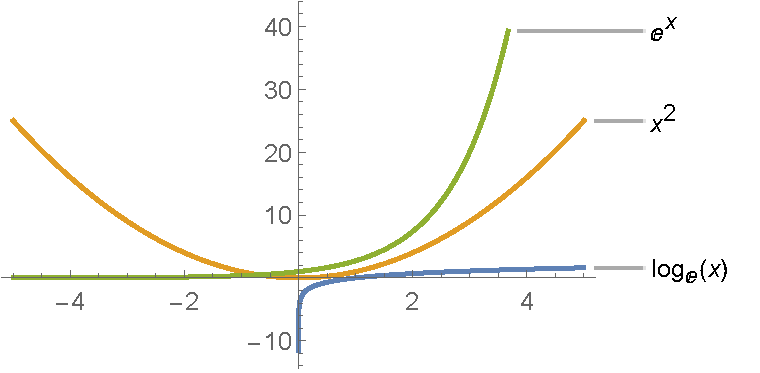
\includegraphics[width=0.5\textwidth]{/0013.pdf}


\subsection{$ \infty + \infty = ? $ 结果未知 } 

\subsection{$ \infty - \infty = ? $ 结果未知 } 

\subsection{$ \infty \cdot \infty = \infty $  } 

\subsection{$ \infty / \infty = ? $ 结果未知 } 





\section{无穷小}

无穷小: 就是``以数0 为极限"的变量。 称一个函数是无穷小量,一定要说明``自变量x"的变化趋势.

\subsection{有限个``无穷小"的和, 是无穷小. } 

\subsection{有限个``无穷小"的乘积, 依然是无穷小. } 

\subsection{常数C × 无穷小 = 无穷小 } 

\subsection{有界函数 × 无穷小 = 无穷小 } 

有界函数, 就是说该函数的"值域", 是在有限区间中的. 如 sin, cos三角函数, 就是有界的.

\begin{myEnvSample}
	\begin{align*}  % 支持每行编号. 若不需要编号, 就用 align*环境
		\begin{matrix}
			\lim_{\text{x}\rightarrow 0}\left( \sin \frac{1}{\text{x}}\cdot \text{x} \right)\\
		\end{matrix}=\begin{matrix}
			\lim_{\text{x}\rightarrow 0}\\
		\end{matrix}\underset{\text{有界函数}}{\underbrace{\left( \sin \frac{1}{\text{x}} \right) }}\cdot \underset{\text{无穷小}}{\underbrace{\begin{matrix}
					\lim_{\text{x}\rightarrow 0}\\
				\end{matrix}\left( \text{x} \right) }}=0 
	\end{align*}
	
	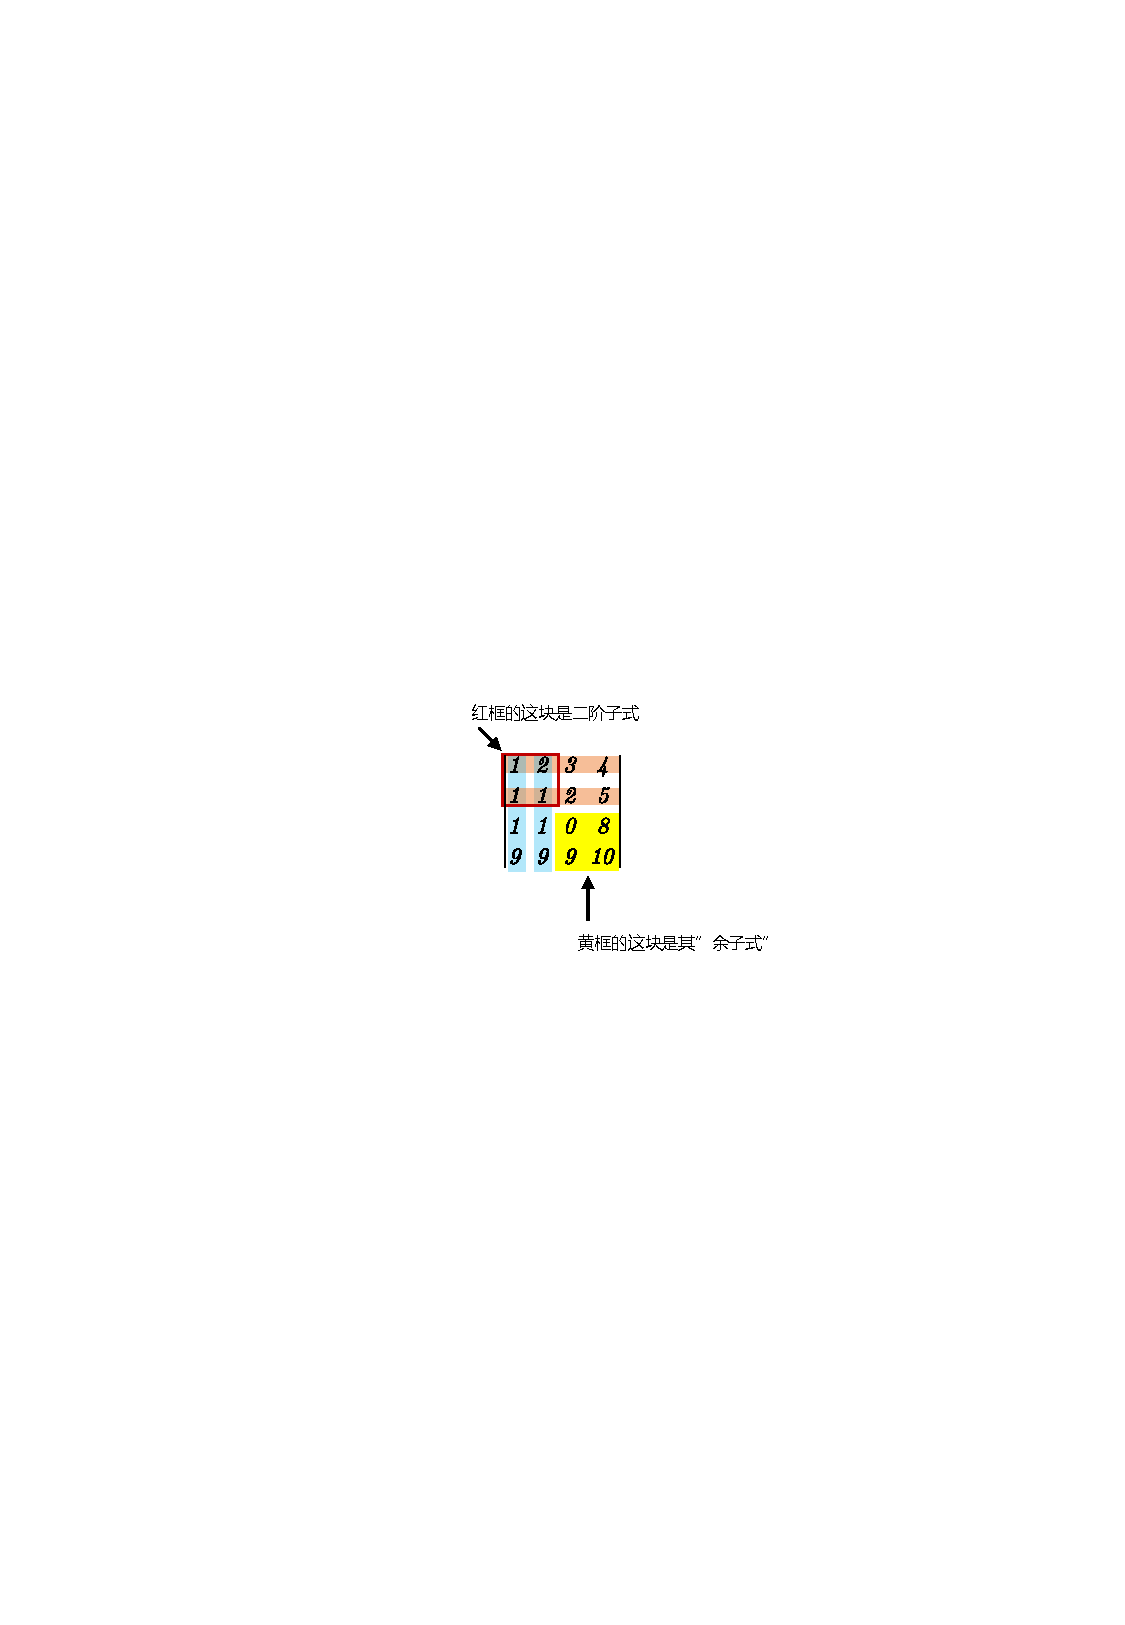
\includegraphics[width=0.5\textwidth]{/0014.pdf}
	
	乘法就意味着: 随着 x → 0, 它把``有界函数"的y值, 越来越压缩到趋向于0. 如下图的中间部分趋势: \\
	
	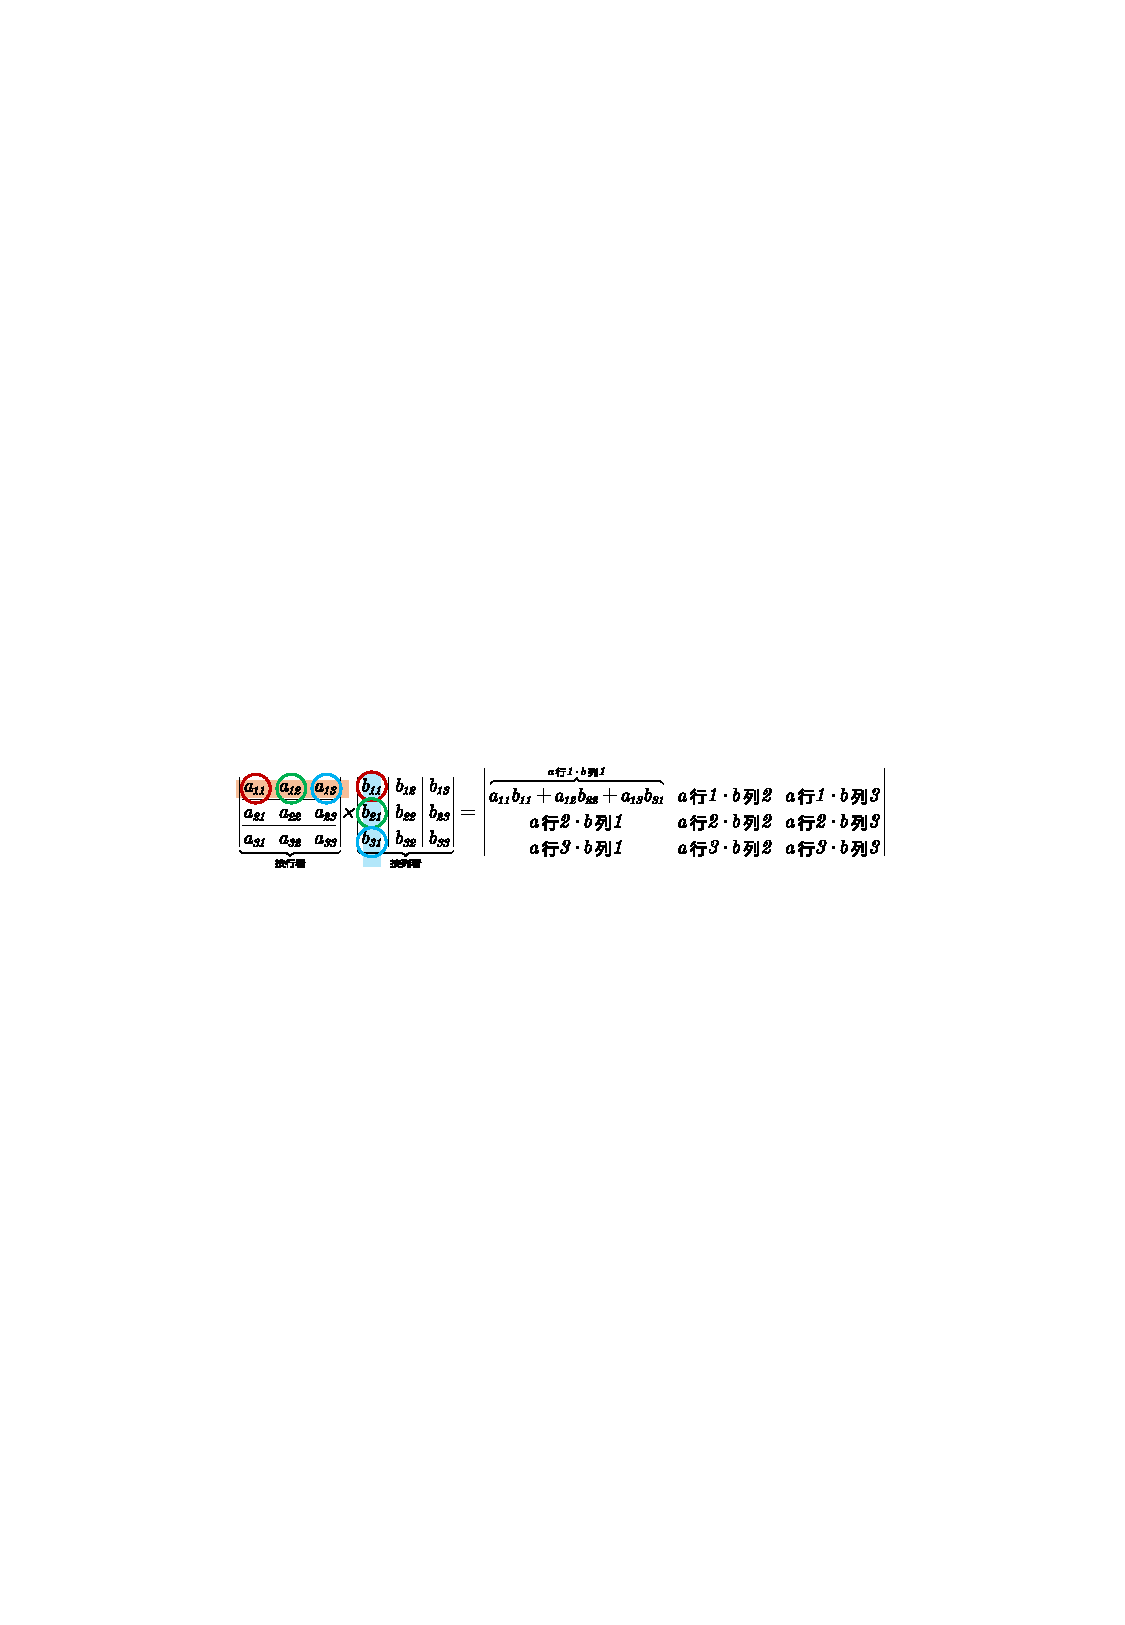
\includegraphics[width=0.5\textwidth]{/0015.pdf}
\end{myEnvSample}


\subsection{无穷小 × 无穷大 = ?  结果未知} 

结果未知. 即可能是无穷小, 也可能是0, 也可能是无穷大.







\section{无穷小的比较 : $ \frac{\text{无穷小}} {\text{无穷小}}$ }

$ \frac{\text{无穷小}} {\text{无穷小}}$ 的比值, 未必是个无穷小, 要看分母和分子,谁缩小地更快.  

两个数都趋向于无穷小 , 但两者趋向于0 的速度有快有慢, 所以它们就能进行比较了.




\subsection{ 高阶无穷小 \& 低阶无穷小} 

对于两个无穷小量 $\alpha$ 和 $\beta$,如果 $\lim \dfrac{\alpha} {\beta}=0$, 我们就把  $\alpha$, 叫做 ``比 $\beta$ 高阶的无穷小量". 简称 ``$\alpha$ 是 $\beta$ 的高阶无穷小  (infinitesimal of higher order)".  意思是 $\alpha \to 0$ 的速度, 远远要比 $\beta \to 0$ 的速度更快.  记作: $\alpha = o(\beta)$  ← 中间的 o 是 希腊字母 omicron.

``高阶"的意思, 就是说``更快速", 即它趋近于0 的速度比别人更快速, 更迅速, 更光速. \\

反过来看, 也就是:  $\beta$ 是``比 $\alpha$ 低阶的无穷小量", 简称:$\beta$ 是  $\alpha$ 的低阶无穷小 ( Low order infinitesimal). 即  $\beta \to 0$  的速度, 要比 $\alpha \to 0$  的速度远远更慢.

即, 如果$\lim \dfrac{\beta} {\alpha} = \infty$, 就称 $\beta$ 是比 $\alpha$ 低阶的无穷小.


\begin{myEnvSample}
$ \lim_{x \to 0} \dfrac{x^2} {3x} = \dfrac{\text{兔子(更快的趋近于0终点)}} {\text{乌龟(更慢的趋近于0终点)}} = 0 \quad \gets $   即 分子 < 分母.  即 $x^2$ 是比 3x ``高阶"的无穷小.

高阶, 即值它趋向于0 的效率 (速度) 更高, 更快. \\


$ \lim_{x \to 0} \dfrac{3x} {x^2} = \dfrac{\text{乌龟(更慢的趋近于0终点)}} {\text{兔子(更快的趋近于0终点)}} = \infty \quad \gets $  即 分子 > 分母.  即 3x 是比 $x^2$ ``低阶"的无穷小. 

低阶, 即值它趋向于0 的效率 (速度) 更低, 更慢. \\

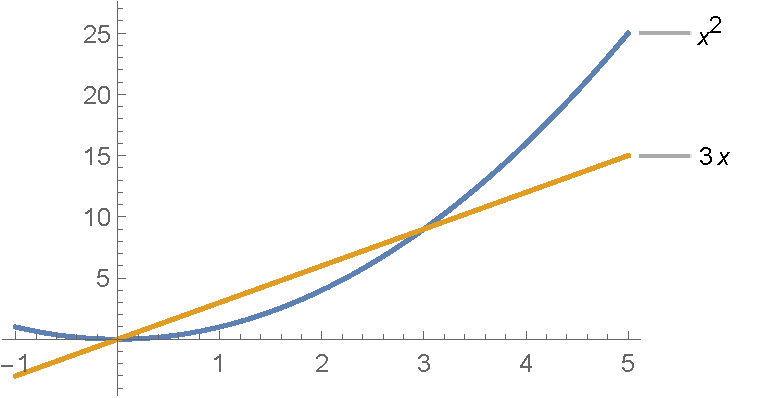
\includegraphics[width=0.5\textwidth]{/0016.pdf}

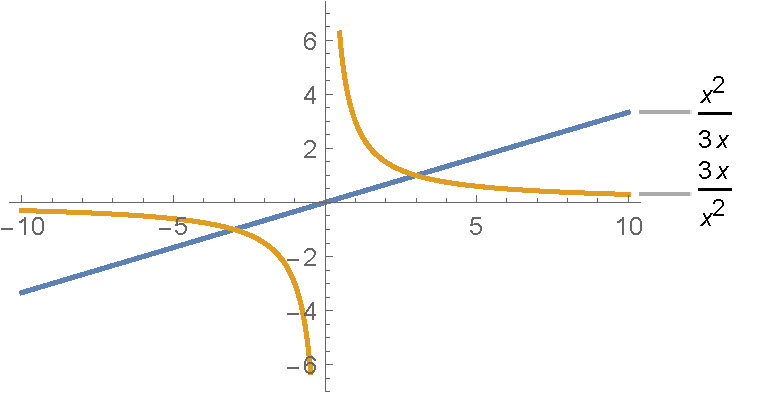
\includegraphics[width=0.5\textwidth]{/0017.pdf}
\end{myEnvSample}




\subsection{同阶无穷小 : $lim \dfrac{b} {a}= \text{常数}C, \quad C \ne 0$} 

若 $\lim \dfrac{b} {a}= \text{常数}C, \quad C \ne 0 $, 就称: b 和 a 为``同阶无穷小" Infinitesimal of the same order. 意思是两者趋近于0的速度相仿。

\begin{myEnvSample}
\begin{align*}  % 支持每行编号. 若不需要编号, 就用 align*环境
	\lim_{\text{x}\rightarrow 0}\frac{\sin\text{x}}{3\text{x}}=\frac{1}{3}  
\end{align*} ← 因为 分子分母的 x的指数次数相同. \\

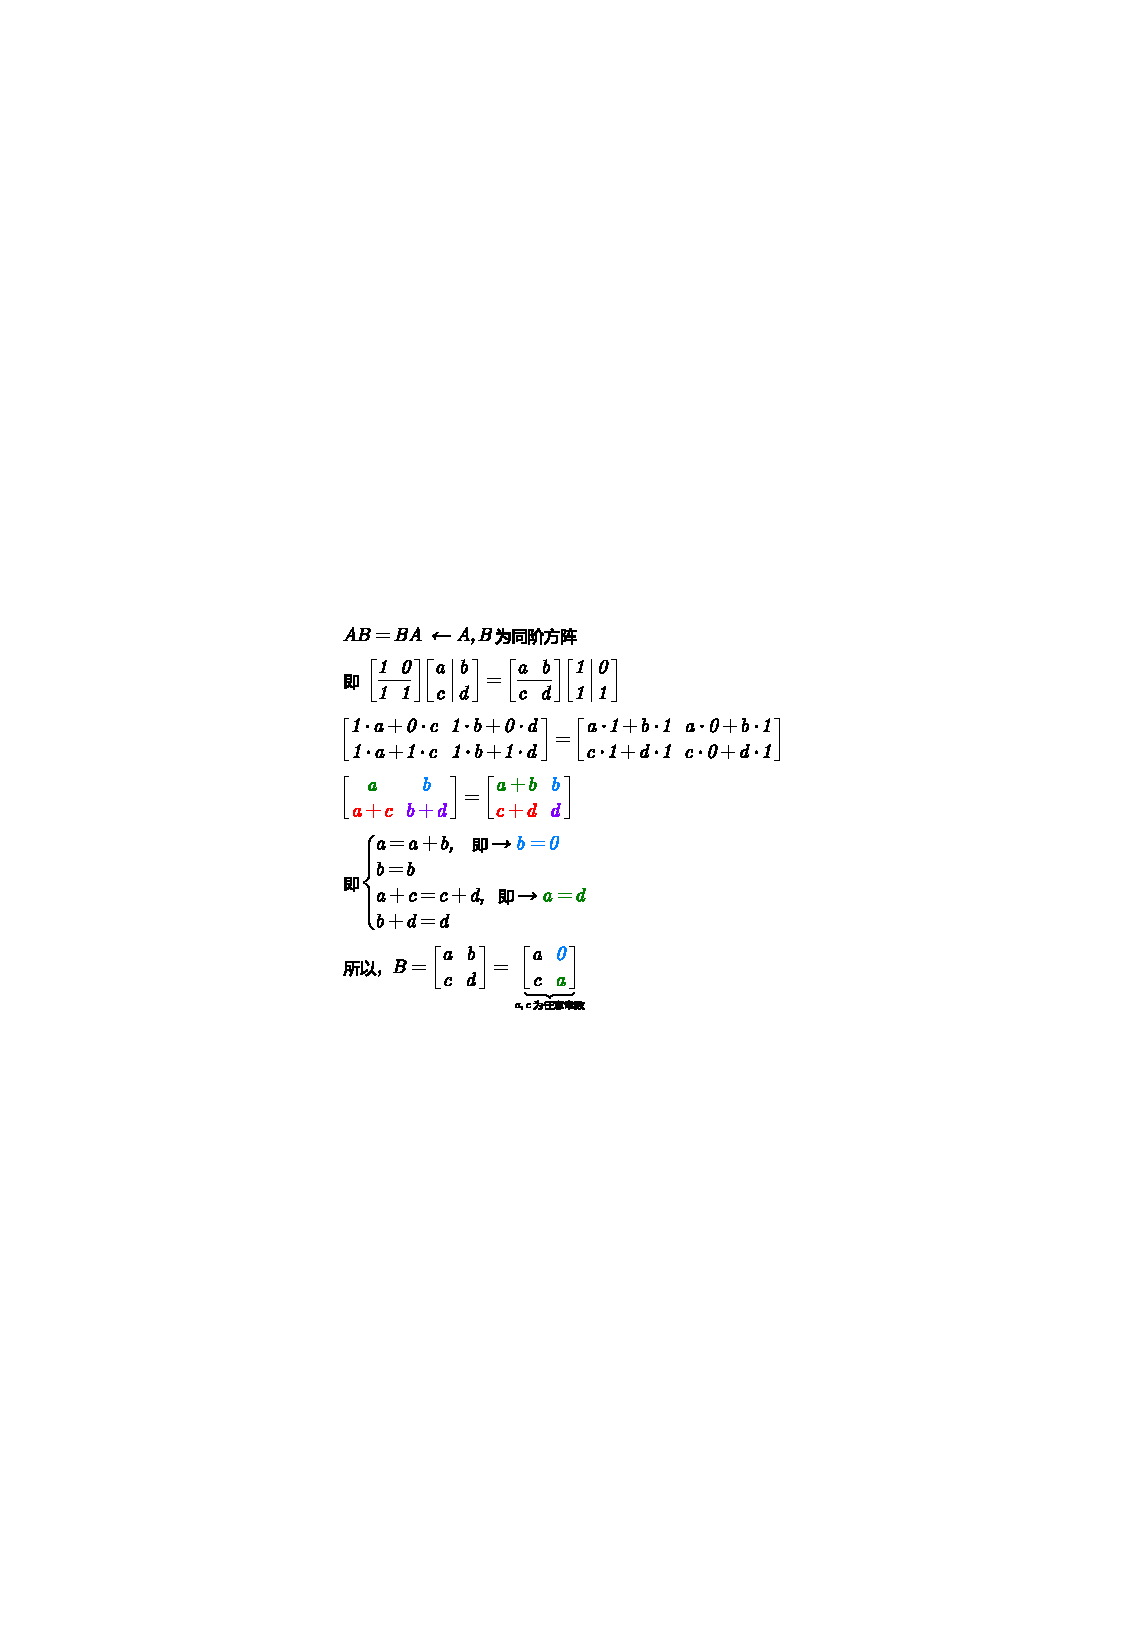
\includegraphics[width=0.5\textwidth]{/0018.pdf}
\end{myEnvSample}






\subsection{等价无穷小 $\to$ $lim \dfrac{b} {a}=1$} 

若 $\lim_{x \rightarrow x_0} \dfrac{\beta} {\alpha} = 1$, 就称: $\beta$ 与 $\alpha$ 是"等价无穷小".记为  $\beta \sim \alpha$ . 等价, 就可以``相互替换"来使用. 

所以我们做题的``方法论"就是: 把复杂的东西, 用它等价的简单东西, 来替换掉. 即, ``以简替繁". \\

注意: 两个函数是``等价无穷小"关系, 因而可以互相替换使用, 这种用法是有前提条件的:

(1) 只有在  $x \to 0$  的时候, 才能用``等价无穷小"的另一种函数来替换.

(2) 只有在求的是 两个``等价无穷小"的``\underline{比值}" 的时候, 才能用``等价物"来替换. 即如果求的是 两个``等价无穷小"的相加, 相减, 相乘, 就都不能用``等价物"来替换. \\

\begin{myEnvSample}
\begin{align*}  % 支持每行编号. 若不需要编号, 就用 align*环境
	&\lim_{\text{x}\rightarrow 0}\frac{\sin\text{x}}{\text{x}^3+3\text{x}}\ \gets \ \text{因为在x}\rightarrow 0\text{时,\ }\sin x \sim x, \text{分子上,\ 我们就用\ x\ 来代替\ }\sin\text{x}\\
	&=\lim_{\text{x}\rightarrow 0}\frac{\text{x}}{\text{x}\left( \text{x}^2+3 \right)}=\lim_{\text{x}\rightarrow 0}\frac{1}{\text{x}^2+3}=\frac{1}{3}
\end{align*}
\end{myEnvSample}


分子或分母, 可拆成若干因子的乘积时, 就可对其中的一个或几个因子, 做等价替换.

注意: 必须是``乘积"才行, 如果只能拆成若干因子的``相加减", 则不能用``等价替换"的方法.




\subsection{ 在 $x \to 0 $时,  $ (1+x)^{\frac{1} {n}} - 1 $ 等价于 $ \dfrac{1} {n} x $ } 


\begin{myEnvSample}
 在$x \to 0 $时, 	$	\left[ \left( 1+x^2 \right) ^{\frac{1}{3}}-1 \right] \sim \left[ \frac{1}{3}x^2 \right] 	$ \\

	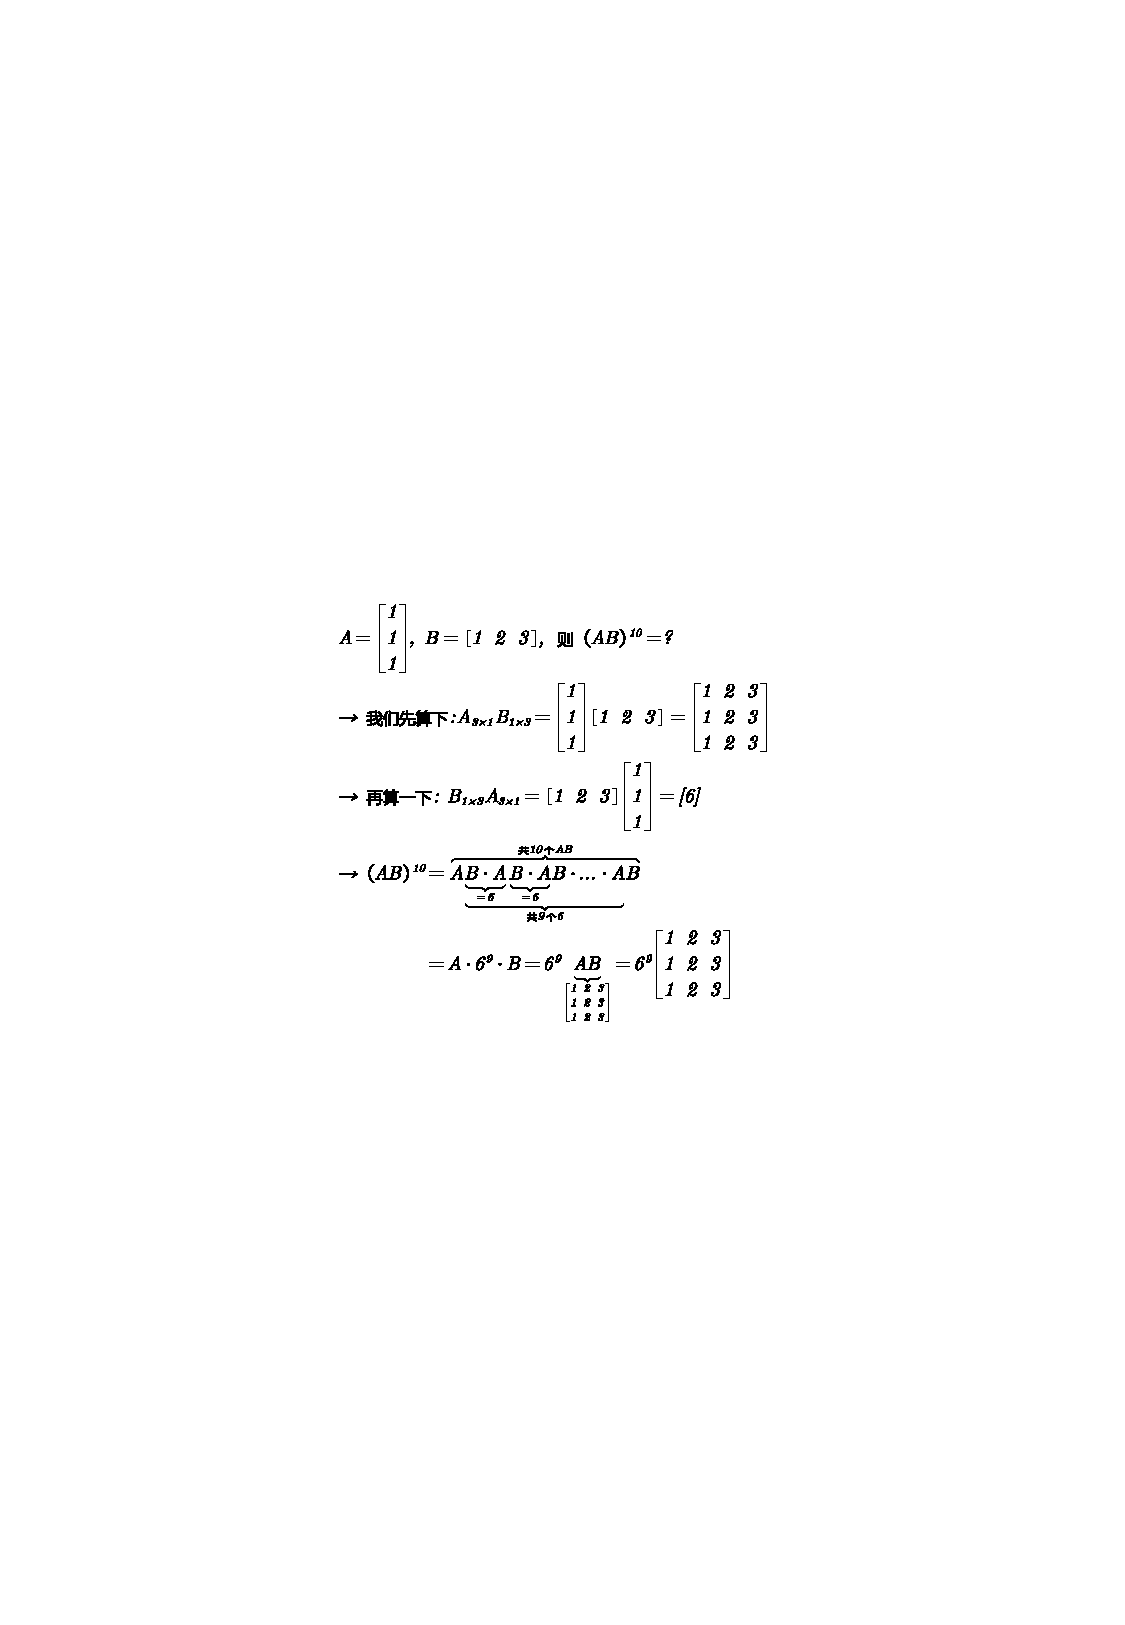
\includegraphics[width=0.5\textwidth]{/0019.pdf}
\end{myEnvSample}




\subsection{k阶无穷小 } 

若 $\lim \dfrac{\beta} {\alpha^k} =  \text{常数}C, \quad C \ne 0,\quad  k>0 $, 就称: $\beta$ 是关于$\alpha$ 的``k阶无穷小".



\end{document}

